\documentclass[12pt]{article}
\usepackage{amsmath}
\usepackage{amssymb}
\usepackage{graphicx}
\usepackage{physics}
\usepackage{hyperref}
\usepackage{tikz}
\usepackage{geometry}
\usepackage[numbers]{natbib}
\bibliographystyle{plainnat}  % or another style like 'apsrev4-2'

\geometry{
    margin=1in,
    textwidth=6.5in,
    textheight=9in
}

\title{Patryk's Notes}
\author{Patryk Kozlowski}
\begin{document}

% Add detailed table of contents settings
\setcounter{tocdepth}{3}  % Show up to subsubsection level in TOC
\tableofcontents
\clearpage  % Start new page after TOC

\maketitle

% Rest of your document content
\section{$G_0W_0$ with k-points: 11/9}
I follow the notation of Tianyu's paper throughout this section \cite{Zhu2020-nt}.
\subsection{Fully analytic}
    We want to solve for the self-energy whose form along the real axis is:
    \begin{equation}
    \Sigma\left(\mathbf{r}, \mathbf{r}^{\prime}, \omega\right)=\frac{i}{2 \pi} \int_{-\infty}^{\infty} e^{i\omega ^{\prime}\eta }d \omega^{\prime} G_{0}\left(\mathbf{r}, \mathbf{r}^{\prime}, \omega+\omega^{\prime}\right) W_{0}\left(\mathbf{r}, \mathbf{r}^{\prime}, \omega^{\prime}\right)
    \end{equation}
    In the molecular brutal basis, the self energy is given as:
    \begin{equation}
        \Sigma_{n n^\prime}(\mathbf{k}, \omega) = \iint d \mathbf{r} d \mathbf{r}^\prime \psi_{n\mathbf{k}}^{*}(\mathbf{r}) \Sigma(\mathbf{r}, \mathbf{r}^\prime, \omega) \psi_{n^\prime\mathbf{k}}(\mathbf{r}^\prime)
    \end{equation}
    Also, recall that the Lehmann representation of the noninteracting Green's function is:
    \begin{equation}
        G_0\left(\mathbf{r}, \mathbf{r}^{\prime}, \omega\right)=\sum_{o \mathbf{q} } \frac{\psi_{o \mathbf{q}}(\mathbf{r}) \psi_{o \mathbf{q}}^{*}\left(\mathbf{r}^{\prime}\right)}{\omega-\epsilon_{o \mathbf{q}}+i \eta \operatorname{sgn}\left(\epsilon_{o \mathbf{q}}-\mu\right)}
    \end{equation}
    Now plugging both of these back into the original expression, we find:


    \begin{align}
        \Sigma_{n n^\prime}(\mathbf{k}, \omega) &= \frac{i}{2 \pi} \sum_{o \mathbf{q}} \int_{-\infty}^{\infty} d \omega^{\prime} \frac{e^{i\omega ^{\prime}\eta }}{\omega + \omega^{\prime} - \epsilon_{o \mathbf{q}} + i \eta \operatorname{sgn}\left(\epsilon_{o \mathbf{q}}-\mu\right)} \nonumber \\
        &\quad \times \iint d \mathbf{r} d \mathbf{r}^\prime \psi_{n\mathbf{k}}^{*}(\mathbf{r}) \psi_{o \mathbf{q}}(\mathbf{r}) W_0(\mathbf{r}, \mathbf{r}^\prime, \omega^{\prime}) \psi_{o \mathbf{q}}^{*}\left(\mathbf{r}^{\prime}\right) \psi_{n^\prime\mathbf{k}}(\mathbf{r}^\prime)\\
        &= \frac{i}{2 \pi} \sum_{o \mathbf{q}} \int_{-\infty}^{\infty} d \omega^{\prime} \frac{e^{i\omega ^{\prime}\eta }}{\omega + \omega^{\prime} - \epsilon_{o \mathbf{k}-\mathbf{q}} + i \eta \operatorname{sgn}\left(\epsilon_{o \mathbf{k}-\mathbf{q}}-\mu\right)} (n_{\mathbf{k}}o_{\mathbf{k-q}}|W_0|o_{\mathbf{k-q}}n^\prime_{\mathbf{k}})
    \end{align}
    Where we have used the fact that the momentum index $\mathbf{q}$ is the same as $\mathbf{k}-\mathbf{q}$, given that we are looping over both $\mathbf{k}$ and $\mathbf{q}$ anyways.


    So the Green's function will bring poles at \(\omega' = \epsilon_{0 \mathbf{k-q}} - \omega+ i\eta\operatorname{sgn}(\mu - \epsilon_{0 \mathbf{k-q}})\).
    Now, we know that the screened Coulomb interaction has the expansion in terms of the bare Coulomb potential \(v\) and the density response function \(\chi_0\) as \(W_0 = v + v\chi_0 v + v\chi_0 v\chi_0 v + \cdots = v\left(1 + \chi_0 v + \chi_0 v \chi_0 v + \cdots\right) = v\left(1 - \chi_0 v\right)^{-1}\), where we recognize the dielectric function as \(\epsilon_0 = 1 - \chi_0 v\) so we can express the screened Coulomb interaction as
    \begin{equation}
    W_0(\mathbf{r}, \mathbf{r}^{\prime}, \omega) = \frac{v(\mathbf{r}, \mathbf{r}^{\prime})}{1 - \left(\chi_0v\right)(\mathbf{r}, \mathbf{r}^{\prime}, \omega)}
    \end{equation}
    recalling that the bare Coulomb interaction should be independent of frequency. A discussion of how to compute the screened Coulomb interaction can be found in this old work \cite{Onida2002-pw}. To simplify notation let us define a polarizability $\boldsymbol{\Pi}\left(\mathbf{r}, \mathbf{r}^{\prime}, \omega\right) = \left(\chi_0 v\right)(\mathbf{r}, \mathbf{r}^{\prime}, \omega)$, so that we can rewrite the screened Coulomb interaction as:
\begin{align}
    (n_{\mathbf{k}}o_{\mathbf{k-q}}|W_0|o_{\mathbf{k-q}}n^\prime_{\mathbf{k}}) = \iint d \mathbf{r} d \mathbf{r}^\prime \psi_{n\mathbf{k}}^{*}(\mathbf{r}) \psi_{o \mathbf{q}}(\mathbf{r}) W_0(\omega ) \psi_{o \mathbf{q}}^{*}\left(\mathbf{r}^{\prime}\right) \psi_{n^\prime\mathbf{k}}(\mathbf{r}^\prime)
\end{align}
At this point, we recognize the decomposition of the ERIs with the Cholesky vectors as:
\begin{equation}
    (p_{\mathbf{k}_p} q_{\mathbf{k}_q} |\frac{1}{|\mathbf{r}-\mathbf{r}^\prime|} |r_{\mathbf{k}_r} s_{\mathbf{k}_s}) = \sum_{PQ} v_{P{\mathbf{q}}}^{p\mathbf{k_p}q\mathbf{k_q}} v_{Q{(\mathbf{-q})}}^{r\mathbf{k_r}s\mathbf{k_s}}
\end{equation}
so each Cholesky brings a factor of $\mathbf{J}^{\frac{1}{2}}$. Each Cholesky is defined as:
\begin{equation}
    v_{P{\mathbf{q}}}^{p\mathbf{k_p}q\mathbf{k_q}} = \sum_{R} \mathbf{J}_{RP}^{-\frac{1}{2}}(\mathbf{q}) \left(R \mathbf{q} \mid p \mathbf{k}_p q \mathbf{k}_q\right)
\end{equation}
where
\begin{equation}
\begin{aligned}
\mathbf{J}_{PQ}(\mathbf{k}) & =\iint d \mathbf{r} d \mathbf{r}^{\prime} \phi_{P(-\mathbf{k})}(\mathbf{r}) \frac{1}{\left|\mathbf{r}-\mathbf{r}^{\prime}\right|} \phi_{Q \mathbf{k}}\left(\mathbf{r}^{\prime}\right) \\
\left(Q \mathbf{k}_{r s} \mid r \mathbf{k}_r s \mathbf{k}_s\right) & =\iint d \mathbf{r} d \mathbf{r}^{\prime} \phi_{Q \mathbf{k}_{r s}}(\mathbf{r}) \frac{1}{\left|\mathbf{r}-\mathbf{r}^{\prime}\right|} \phi_{r \mathbf{k}_r}^*\left(\mathbf{r}^{\prime}\right) \phi_{s \mathbf{k}_s}\left(\mathbf{r}^{\prime}\right)
\end{aligned}
\end{equation}
So the simplest thing now will be to derive an expression for the columb interaction in terms of an auxiliary basis:
\begin{equation}
W_{0, PQ}(\omega)=\left[\mathbf{J}(\mathbf{I}-\mathbf{\Pi}(\mathbf{q}, \omega))^{-1}\right]_{PQ}
\end{equation}
and then we need to contract with the Choleskies to get the matrix element:
\begin{equation}
    (n_{\mathbf{k}}o_{\mathbf{k-q}}|W_0|o_{\mathbf{k-q}}n^\prime_{\mathbf{k}}) =\sum_{PQ} v_{P}^{nm}\left[\mathbf{I}-\mathbf{\Pi}\left(\mathbf{q}, \omega\right)\right]_{PQ}^{-1} v_{Q}^{mn^{\prime}}
\end{equation}

So in our quest to find poles of $W_0$, we are really just looking for poles of the $\chi_0$. $\chi_0$ is given by:
\begin{equation}
\chi_{0}\left(\mathbf{r}, \mathbf{r}^{\prime}, \omega\right)=\sum_{r\mathbf{k} s \mathbf{k}^{\prime}}\left(f_{r \mathbf{k}}-f_{s \mathbf{k}^{\prime}}\right) \frac{\psi_{r \mathbf{k}}(\mathbf{r}) \psi_{r \mathbf{k}}^{*}\left(\mathbf{r}^{\prime}\right) \psi_{s \mathbf{k}^{\prime}}\left(\mathbf{r}^{\prime}\right) \psi_{s \mathbf{k}^{\prime}}^{*}(\mathbf{r})}{\omega-\left(\epsilon_{r \mathbf{k}}-\epsilon_{s \mathbf{k}^{\prime}}\right)+i \eta \operatorname{sgn}\left(\epsilon_{r \mathbf{k}}-\epsilon_{s \mathbf{k}^{\prime} } - \mu\right)}
\end{equation}
where the occupations of the KS states \(r\mathbf{k}(s\mathbf{k}^{\prime})\) with energies \(\epsilon_{r\mathbf{k}}(\epsilon_{s\mathbf{k}^{\prime}})\) are given by the Fermi-Dirac distribution \(f_{r\mathbf{k}}(f_{s\mathbf{k}^{\prime}})\), which is just a step function at zero temperature. Notice that the occupation factor will always be 0 unless \(rs\) form an occupied-virtual pair. So we can separate the density response into two terms, one where \(\delta_{ri}\) and \(\delta_{sa}\) and the other with \(\delta_{ra}\) and \(\delta_{si}\), where \(i\) and \(a\) are occupied and virtual indices, respectively. This allows us to now combine with the bare Coulomb potential in order to form the polarizability \(\Pi\equiv \chi_0v\) as:
\begin{equation}
\Pi\left(\mathbf{r}, \mathbf{r}^{\prime}, \omega\right)=\sum_{i\mathbf{k}a\mathbf{k}^{\prime}}\frac{\psi_{i\mathbf{k}}(\mathbf{r}) \psi_{i\mathbf{k}}^{*}\left(\mathbf{r}^{\prime}\right)\frac{1}{|\mathbf{r}-\mathbf{r}^\prime|} \psi_{a\mathbf{k}^{\prime}}\left(\mathbf{r}^{\prime}\right) \psi_{a\mathbf{k}^{\prime}}^{*}(\mathbf{r})}{\omega+\left(\Omega_{i\mathbf{k}a\mathbf{k}^{\prime}}\right)-i\eta } - \sum_{a\mathbf{k}i\mathbf{k}^{\prime}}\frac{\psi_{a\mathbf{k}}(\mathbf{r}) \psi_{a\mathbf{k}}^{*}\left(\mathbf{r}^{\prime}\right) \frac{1}{|\mathbf{r}-\mathbf{r}^\prime|}\psi_{i\mathbf{k}^{\prime}}\left(\mathbf{r}^{\prime}\right) \psi_{i\mathbf{k}^{\prime}}^{*}(\mathbf{r})}{\omega-\left(\Omega_{i\mathbf{k}a\mathbf{k}^{\prime}}\right)+i\eta },
\end{equation}
where we define the KS eigenvalue differences as \(\Omega_{i\mathbf{k}a\mathbf{k}^{\prime}} = \epsilon_{a\mathbf{k}} - \epsilon_{i\mathbf{k}^{\prime}}\), which will eventually become the excitation energies from RPA. So sandwiching this operator in between the molecular or brutal bases gives:
\begin{equation}
    \bra{n\mathbf{k}} \Pi (\omega) \ket{n^\prime\mathbf{k}} = \sum_{iajb \mathbf{k} \mathbf{k}^{\prime}} \frac{(ia\mid jb)}{(\omega + \Omega ^{\mu}_{\mathbf{k}})-i\eta} - \sum_{aibj \mathbf{k} \mathbf{k}^{\prime}} \frac{(ai\mid bj)}{(\omega - \Omega ^{\mu}_{\mathbf{k}})+i\eta}
\end{equation}
\emph{So we see that we can get the poles of the screened Coulomb interaction by the poles of the polarizability, which are \(\omega = \Omega ^{\mu}_{\mathbf{k}} - i\eta\) and \(\omega = \Omega ^{\mu}_{\mathbf{k}} + i\eta\), suggesting that they are in the upper complex plane for excitations and vice versa for deexcitations.} See the figure \ref{fig:contour} for a picture. For a more comprehensive picture, this should be juxtaposed with the figure from Tianyu's paper for CD. In the literature, they talk about approximating the dielectric function by a multiple one or a single pole approximation, so which one would I want to implement? This suggests that the notation in the \(G_0W_0\) literature is confusing because they always say that to solve for the \(\chi_0\) in the RPA, but if we are actually dealing with \(\chi_0\), which is the Kohn-Sham density response function, then we don't use the RPA, where the density response function is solved for using a Dyson-like equation \cite{Sander2015-xq}:
    \begin{figure}[h]
    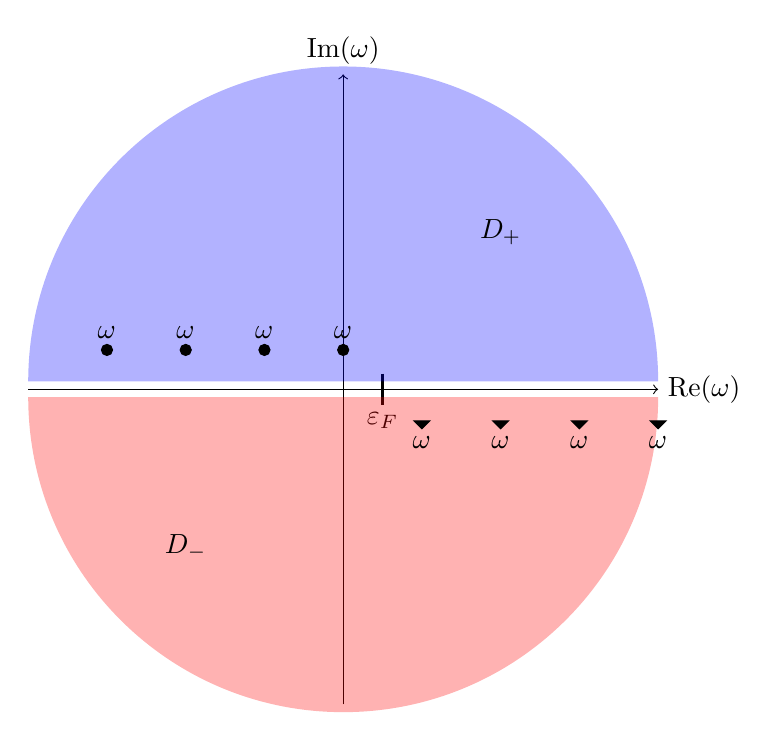
\begin{tikzpicture}
    % Draw the axes
    \draw[->] (-4, 0) -- (4, 0) node[right] {Re($\omega$)};
    \draw[->] (0, -4) -- (0, 4) node[above] {Im($\omega$)};
    
    % Draw the positive real axis label and tick mark for \varepsilon_{F}
    \draw[thick] (0.5, 0.2) -- (0.5, -0.2);
    \node at (0.5, -0.4) {$\varepsilon_{F}$};


    % Draw the semicircle contours
    % fill in its under side
    \fill[blue, opacity=0.3] (4, 0.1) arc[start angle=0, end angle=180, radius=4];
    \fill[red, opacity=0.3] (4, -0.1) arc[start angle=0, end angle=-180, radius=4];
    
    % Draw the poles above the real axis
    \foreach \x in {-3,-2,-1,0} {
        \draw[fill=black] (\x, 0.5) circle (2pt);
    }
    \node at (-3, 0.7) {$\omega_{}$};
    \node at (-2, 0.7) {$\omega_{}$};
    \node at (-1, 0.7) {$\omega_{}$};
    \node at (0, 0.7) {$\omega_{}$};    

    % Draw the poles below the real axis
    \foreach \x in {1,2,3,4} {
        \draw[fill=black] (\x, -0.5) -- ++(0.1, 0.1) -- ++(-0.2, 0) -- cycle;
    }
    \node at (1, -0.7) {$\omega_{}$};
    \node at (2, -0.7) {$\omega_{}$};
    \node at (3, -0.7) {$\omega_{}$};
    \node at (4, -0.7) {$\omega_{}$};

    
    % Label the contours
    \node at (2, 2) {$D_+$};
    \node at (-2, -2) {$D_-$};
    \end{tikzpicture}
    \caption{Contour for the complex frequency integral. The poles are denoted by the various $\omega$. The Fermi energy is denoted by $\varepsilon_F$. The integration contour $D_+$ is the semicircle in the upper complex plane, while $D_-$ is the semicircle in the lower complex plane.}
    \label{fig:contour}
    \end{figure}
\begin{equation}\label{eq:dyson}
    \chi^{\lambda}\left(\mathbf{r}, \mathbf{r}^{\prime}, i \omega\right) = \chi^{0}\left(\mathbf{r}, \mathbf{r}^{\prime}, i \omega\right) 
    + \int d \mathbf{r}_{1} d \mathbf{r}_{2} \chi^{0}\left(\mathbf{r}, \mathbf{r}_{1}, i \omega\right)\left[\frac{\lambda}{\left|\mathbf{r}_{1}-\mathbf{r}_{2}\right|}+f_{\mathrm{xc}}^{\lambda}\left(\mathbf{r}_{1}, \mathbf{r}_{2}, i \omega\right)\right] \chi^{\lambda}\left(\mathbf{r}_{2}, \mathbf{r}^{\prime}, \omega\right)
\end{equation}
where the parameter $\lambda$ controls the amount of interaction in the system, ranging from $\lambda = 0$ for the KS reference system to $\lambda = 1$ for the fully interacting system. The $f_{\mathrm{xc}}^{\lambda}$ is the exchange-correlation kernel, which is set to zero for the RPA. But we will proceed with an RPA calculation anyways in order to solve for the excitation energies and their corresponding eigenvectors. So it makes sense that the numerator of the expression for the screened Coulomb interaction should be given a construction of the ERIs with the excitation factors in a transition density defined as:
\begin{equation}
    w_{pq}^{\mu} = \sum_{ia} (pq|ia) \left(X_{ia}^{\mu} + Y_{ai}^{\mu}\right)
\end{equation}
where we have defined the excitation and de-excitation vectors at the excitation index $\mu$ as $X_{ia}^{\mu}$ and $Y_{ai}^{\mu}$, respectively.
I am not sure how to connect this with the known expression $v\epsilon ^{-1}$; I see the similarities given that we are contracting an ERI with what we get from the RPA calculation that is connected to the polarizability, but can't connect exactly.
We want to figure out how this matches with my previous $O(N^6)$ expression, which was
\begin{equation}
    \Sigma_{pp}^{\text{corr}}(\omega) = \sum_{\mu }^{\text{RPA}}\left(\sum_{i}^{\text{occupied}} \frac{w_{pi}^{\mu }w_{ip}^{\mu }}{\omega -(\epsilon _{i}-\Omega  _{\mu })}+ \sum_{a}^{\text{virtual}} \frac{w_{pa}^{\mu }w_{ap}^{\mu }}{\omega -(\epsilon _{a}+\Omega  _{\mu })}\right)
\end{equation}
for the molecular case. Today I want us to dissect how this equation came about, so that I can understand for my k-point version.
% The expression I get adapted for k-points from GPT is:
% \begin{equation}
% \Sigma_{n n^\prime}^{\text {corr }}(\mathbf{k}, \omega)=\sum_{\mathbf{q}} \sum_\mu^{\text {RPA }}\left(\sum_i^{\text {occupied }} \frac{w_{n i}^\mu(\mathbf{k}, \mathbf{q}) w_{i n^\prime}^\mu(\mathbf{k}-\mathbf{q}, \mathbf{q})}{\omega-\left(\epsilon_{i, \mathbf{k}-\mathbf{q}}-\Omega_{\mu, \mathbf{q}}\right)}+\sum_a^{\text {virtual }} \frac{w_{n a}^\mu(\mathbf{k}, \mathbf{q}) w_{a n^\prime}^\mu(\mathbf{k}-\mathbf{q}, \mathbf{q})}{\omega-\left(\epsilon_{a, \mathbf{k}-\mathbf{q}}+\Omega_{\mu, \mathbf{q}}\right)}\right)
% \end{equation}

\subsection{Analytic continuation}
\label{sec:analytic_continuation}
We start with the original form for the self-energy along the real axis:
\begin{equation}
\Sigma\left(\mathbf{r}, \mathbf{r}^{\prime}, \omega\right)=\frac{i}{2 \pi} \int_{-\infty}^{\infty} d \omega^{\prime} e^{i \omega^{\prime} \eta} G_{0}\left(\mathbf{r}, \mathbf{r}^{\prime}, \omega+\omega^{\prime}\right) W_{0}\left(\mathbf{r}, \mathbf{r}^{\prime}, \omega^{\prime}\right)
\end{equation}
But to avoid the poles, we need to evaluate along the imaginary axis, so the problem becomes:
\begin{equation*}
\Sigma\left(\mathbf{r}, \mathbf{r}^{\prime}, i \omega\right)=-\frac{1}{2 \pi} \int_{-\infty}^{\infty} d \omega^{\prime} G_{0}\left(\mathbf{r}, \mathbf{r}^{\prime}, i \omega+i \omega^{\prime}\right) W_{0}\left(\mathbf{r}, \mathbf{r}^{\prime}, i \omega^{\prime}\right) 
\end{equation*}
We are interested in evaluating the matrix elements of this operator in the molecular orbital basis. Note that both molecular orbitals must have the same crystal momentum in order for it to be conserved in this process. We also apply the identity operator:
\begin{equation}
\bra{n\mathbf{k}} \Sigma (i \omega) \ket{n^\prime\mathbf{k}} = -\frac{1}{2 \pi} \sum_{m\mathbf{k}^\prime}\int_{-\infty}^{\infty} d \omega^{\prime} \bra{n\mathbf{k}} G_0(i \omega + i \omega^{\prime}) \ket{m\mathbf{k^\prime}}\bra{m\mathbf{k^\prime}}W_0(i \omega^{\prime}) \ket{n^\prime\mathbf{k}}
\end{equation}
The noninteracting Green's function has the form:
\begin{equation*}
G_{0}\left(\mathbf{r}, \mathbf{r}^{\prime}, i \omega\right)=\sum_{m \mathbf{k}_{m}} \frac{\psi_{m \mathbf{k}_{m}}(\mathbf{r}) \psi_{m \mathbf{k}_{m}}^{*}\left(\mathbf{r^\prime}\right)}{i \omega+\epsilon_{F}-\epsilon_{m \mathbf{k}_{m}}} \implies G_{0}\left(\mathbf{k} - \mathbf{q}, i \omega + i \omega^{\prime}\right) = \sum_{m \mathbf{k}-\mathbf{q}} \frac{\psi_{m \mathbf{k}-\mathbf{q}} \psi_{m \mathbf{k}-\mathbf{q}}^{*}}{i \left(\omega + \omega^{\prime}\right) + \epsilon_{F} - \epsilon_{m \mathbf{k}-\mathbf{q}}}
\end{equation*}
so that the above equation simplifies to:
\begin{equation}
\boldsymbol{\Sigma}_{n n^{\prime}}(\mathbf{k}, i \omega) = -\frac{1}{2 \pi N_{\mathbf{k}}} \sum_{m \mathbf{q}} \int_{-\infty}^{\infty} d \omega^{\prime} \frac{(n\mathbf{k}, m\mathbf{k}-\mathbf{q} \mid W_0 (\mathbf{q}, i\omega )\mid m \mathbf{k}-\mathbf{q}, n^{\prime}\mathbf{k})}{i \left(\omega + \omega^{\prime}\right) + \epsilon_{F} - \epsilon_{m \mathbf{k}-\mathbf{q}}}
\end{equation}
\subsubsection{Screened Coulomb Interaction}
\begin{align*}
\left(n\mathbf{k}, m\mathbf{k}-\mathbf{q}\left|W_{0}(\mathbf{q}, i\omega )\right| m\mathbf{k}-\mathbf{q}, n^{\prime}\mathbf{k}\right) &= \int \int d \mathbf{r}_1 d \mathbf{r}_2 \psi_{n\mathbf{k}}^{*}(\mathbf{r}_1) \psi_{m\mathbf{k}-\mathbf{q}}(\mathbf{r}_1) W_0(\mathbf{q}, \mathbf{r}_1, \mathbf{r}_2, i\omega ) \psi_{m\mathbf{k}-\mathbf{q}}^{*}(\mathbf{r}_2) \psi_{n^{\prime}\mathbf{k}}(\mathbf{r}_2) \\
\end{align*}
We expand the orbital pair product $\psi_{n \mathbf{k}}^{*}(\mathbf{r}) \psi_{m \mathbf{k}-\mathbf{q}}(\mathbf{r})$ in the auxiliary basis

\begin{equation*}
\psi_{n \mathbf{k}}^{*}(\mathbf{r}) \psi_{m \mathbf{k}-\mathbf{q}}(\mathbf{r})=\sum_{P} b_{P \mathbf{q}}^{n \mathbf{k}, m \mathbf{k}-\mathbf{q}} \phi_{P \mathbf{q}}(\mathbf{r}) 
\end{equation*}
and
\begin{equation}
    \psi_{m\mathbf{k}-\mathbf{q}}^{*}(\mathbf{r}) \psi_{n^{\prime}\mathbf{k}}(\mathbf{r}) = \sum_{Q} b_{Q(-\mathbf{q})}^{m\mathbf{k}-\mathbf{q}, n^{\prime}\mathbf{k}} \phi_{Q(-\mathbf{q})}(\mathbf{r})
\end{equation}
where we have recognized the fact that in the former there is a momentum transfer of $\mathbf{q}$, and in the latter, there is a momentum transfer of $-\mathbf{q}$.
Substituting in gives
\begin{align}
    \left(n\mathbf{k}, m\mathbf{k}-\mathbf{q}\left|W_{0}(\mathbf{q}, i\omega )\right| m\mathbf{k}-\mathbf{q}, n^{\prime}\mathbf{k}\right)\\ = \sum_{PQ} b_{P\mathbf{q}}^{n\mathbf{k}, m\mathbf{k}-\mathbf{q}} \left[\iint d\mathbf{r}_1 d\mathbf{r}_2 \phi_{P\mathbf{q}}(\mathbf{r}_1) W_0(\mathbf{q}, \mathbf{r}_1, \mathbf{r}_2, i\omega ) \phi_{Q(-\mathbf{q})}(\mathbf{r}_2)\right] b_{Q(-\mathbf{q})}^{m\mathbf{k}-\mathbf{q}, n^{\prime}\mathbf{k}}
\end{align}
with

\begin{equation}
b_{P \mathbf{q}}^{n \mathbf{k}, m \mathbf{k}-\mathbf{q}}=\sum_{R}(n \mathbf{k}, m \mathbf{k}-\mathbf{q} \mid R \mathbf{q}) \cdot \mathbf{J}_{R P}^{-1}(\mathbf{q})
\label{eq:nonchol}
\end{equation}
Now is a good place to recall their definition of the density fitting where the ERIs are represented as:


\begin{equation*}
\left(p \mathbf{k}_{p} q \mathbf{k}_{q} \mid r \mathbf{k}_{r} s \mathbf{k}_{s}\right)=\sum_{P Q}\left(p \mathbf{k}_{p} q \mathbf{k}_{q} \mid P \mathbf{k}_{p q}\right) \mathbf{J}_{P Q}^{-1}\left(Q \mathbf{k}_{r s} \mid r \mathbf{k}_{r} s \mathbf{r}_{s}\right), 
\end{equation*}
with
\begin{align*}
\mathbf{J}_{P Q}(\mathbf{k}) & =\iint d \mathbf{r} d \mathbf{r}^{\prime} \phi_{P(-\mathbf{k})}(\mathbf{r}) \frac{1}{\left|\mathbf{r}-\mathbf{r}^{\prime}\right|} \phi_{Q \mathbf{k}}\left(\mathbf{r}^{\prime}\right),  \\
\left(Q \mathbf{k}_{r s} \mid r \mathbf{k}_{r} s \mathbf{k}_{s}\right) & =\iint d \mathbf{r} d \mathbf{r}^{\prime} \phi_{Q \mathbf{k}_{r s}}(\mathbf{r}) \frac{1}{\left|\mathbf{r}-\mathbf{r}^{\prime}\right|} \phi_{r \mathbf{k}_{r}}^{*}\left(\mathbf{r}^{\prime}\right) \phi_{s \mathbf{k}_{s}}\left(\mathbf{r}^{\prime}\right) . 
\end{align*}
Note that these $b$ are then not yet our Cholesky vectors, since each one contains $\frac{|\mathbf{r}-\mathbf{r}^{\prime}|}{|\mathbf{r}-\mathbf{r}^{\prime}|}$ scaling, i.e., there should be a factor of $\mathbf{J}^{-\frac{1}{2}}$  instead of $\mathbf{J}^{-1}$ in \ref{eq:nonchol} if we are to apply the Cholesky vectors.
At this point, we use the expansion of the screened Coulomb interaction:
\begin{align}
    W_0 &= v + v\chi_0 v + v\chi_0 v\chi_0 v + \cdots\\
    &= v(1 + \chi_0 v + \chi_0 v \chi_0 v + \cdots)\\
    &= v^{1/2} \left(1 - \chi_0\right)^{-1} v^{1/2}
\end{align}
simplifying to 
\begin{align}
    \left(n\mathbf{k}, m\mathbf{k}-\mathbf{q}\left|W_{0}(\mathbf{q}, i\omega )\right| m\mathbf{k}-\mathbf{q}, n^{\prime}\mathbf{k}\right) &= \sum_{PQ} b_{P\mathbf{q}}^{n\mathbf{k}, m\mathbf{k}-\mathbf{q}} \left[\mathbf{J^{\frac{1}{2}}}\left( \mathbf{I} - \boldsymbol{\Pi}(\mathbf{q}, i\omega ) \right) \mathbf{J^{\frac{1}{2}}}\right]^{-1}_{PQ} b_{Q(-\mathbf{q})}^{m\mathbf{k}-\mathbf{q}, n^{\prime}\mathbf{k}}\\
    &= \sum_{PQ} v_{P}^{n m}\left[\mathbf{I}-\mathbf{\Pi}\left(\mathbf{q}, i \omega^{\prime}\right)\right]_{P Q}^{-1} v_{Q}^{m n^{\prime}}
\end{align}
where $\mathbf{J}_{PQ}$ is the Coulomb interaction projected onto the auxiliary basis, and we have defined
\begin{equation}
    v_{P\mathbf{q}}^{n \mathbf{k}, m \mathbf{k}-\mathbf{q}} = \sum_{pq} C_{pn}(\mathbf{k}) C_{qm}(\mathbf{k}-\mathbf{q}) v_{P\mathbf{q}}^{p\mathbf{k}, q\mathbf{k}-\mathbf{q}}
\label{eq:mochol}
\end{equation}
with
\begin{equation}
    v_{P\mathbf{q}}^{p\mathbf{k}, q\mathbf{k}-\mathbf{q}} = \sum_R (p\mathbf{k}, q\mathbf{k}-\mathbf{q} \mid R\mathbf{q}) \mathbf{J}_{RP}^{-1/2}(\mathbf{q})
\end{equation}
If we first rename $\mathbf{k^\prime} = \mathbf{k}-\mathbf{q} \implies \mathbf{k} = \mathbf{k^\prime} + \mathbf{q}$, and then we are free to redefine $\mathbf{q} \rightarrow -\mathbf{q}$, so that \ref{eq:mochol} becomes
\begin{equation}
    v_{P\mathbf{-q}}^{n \mathbf{k}-\mathbf{q}, m \mathbf{k}} = \sum_{pq} C_{pn}(\mathbf{k}-\mathbf{q}) C_{qm}(\mathbf{k}) v_{P\mathbf{-q}}^{p\mathbf{k}-\mathbf{q}, q\mathbf{k}}
\end{equation}
but we know that the bare Coulomb potential projected onto the auxiliary basis is given by
\begin{equation}
    v_{P\mathbf{q}}^{n\mathbf{k}, m\mathbf{k}-\mathbf{q}} = \sum_{pq} C_{pn}(\mathbf{k}) C_{qm}(\mathbf{k}-\mathbf{q}) v_{P\mathbf{q}}^{p\mathbf{k}, q\mathbf{k}-\mathbf{q}}
\end{equation}

To ease notation, some momentum labels are suppressed in the above and following equations (e.g., we will use $b_{P}^{n m}$ to denote $b_{P \mathbf{q}}^{n \mathbf{k}, m \mathbf{k}-\mathbf{q}}$ ). Using Eqs. 19-21, the matrix elements of $W_{0}$ are computed as

\begin{align*}
& \left(n \mathbf{k}, m \mathbf{k}-\mathbf{q}\left|W_{0}\right| m \mathbf{k}-\mathbf{q}, n^{\prime} \mathbf{k}\right) \\
& =\sum_{P Q} b_{P}^{n m}\left[\iint d \mathbf{r} d \mathbf{r}^{\prime} \phi_{P \mathbf{q}}(\mathbf{r}) W_{0}\left(\mathbf{r}, \mathbf{r}^{\prime}, i \omega^{\prime}\right) \phi_{Q(-\mathbf{q})}\left(\mathbf{r}^{\prime}\right)\right] b_{Q}^{m n^{\prime}} \\
& =\sum_{P Q} b_{P}^{n m}\left[\mathbf{J}_{P Q}(\mathbf{q})+\left(\mathbf{J}^{1 / 2} \boldsymbol{\Pi} \mathbf{J}^{1 / 2}\right)_{P Q}(\mathbf{q})+\ldots\right] b_{Q}^{m n^{\prime}}  \\
& =\sum_{P Q} v_{P}^{n m}\left[\mathbf{I}-\mathbf{\Pi}\left(\mathbf{q}, i \omega^{\prime}\right)\right]_{P Q}^{-1} v_{Q}^{m n^{\prime}}
\end{align*}

The 3-center 2-electron integral $v_{P}^{n m}$ between auxiliary basis function $P$ and molecular orbital pairs $n m$ is obtained from an AO to MO transformation of the GDF AO integrals defined in Eq. 15:

\begin{equation*}
v_{P}^{n m}=\sum_{p} \sum_{q} C_{p n}(\mathbf{k}) C_{q m}(\mathbf{k}-\mathbf{q}) v_{P \mathbf{q}}^{p \mathbf{k}, q \mathbf{k}-\mathbf{q}} 
\end{equation*}

where $C(\mathbf{k})$ refers to the MO coefficients in the AO basis. $\Pi\left(\mathbf{q}, i \omega^{\prime}\right)$ in Eq. 22 is an auxiliary density response function:

\begin{equation*}
\boldsymbol{\Pi}_{P Q}\left(\mathbf{q}, i \omega^{\prime}\right)=\frac{2}{N_{\mathbf{k}}} \sum_{\mathbf{k}} \sum_{i}^{\mathrm{occ}} \sum_{a}^{\text {vir }} v_{P}^{i a} \frac{\epsilon_{i \mathbf{k}}-\epsilon_{a \mathbf{k}-\mathbf{q}}}{\omega^{\prime 2}+\left(\epsilon_{i \mathbf{k}}-\epsilon_{a \mathbf{k}-\mathbf{q}}\right)^{2}} v_{Q}^{a i} 
\end{equation*}
\section{$G_0W_0$ Derivation: 11/16}
We follow the Subotnik paper \cite{Ou2016-ti}. 
\subsection{Just the formulas}
The first thing to do is to solve the Casida equation for the polarizability in the direct formulation of the RPA:
\begin{equation}\label{eq:kptsCasida}
	\begin{pmatrix}
        \mathbf{A}  & \mathbf{B} \\
        \mathbf{B}^{*} & \mathbf{A}^{*}
    \end{pmatrix}
    \begin{pmatrix}
        \mathbf{X} \\
        \mathbf{Y}
    \end{pmatrix}
    =
    \begin{pmatrix}
        \Omega & 0 \\
        0 & -\Omega
    \end{pmatrix}
    \begin{pmatrix}
        \mathbf{X} \\
        \mathbf{Y}
    \end{pmatrix}
\end{equation}
with $\mathbf{A}$ and $\mathbf{B}$ given by
    \begin{align}\nonumber
    \mathbf{A}_{ia, jb}^{\sigma \sigma ^{\prime}} &= \delta_{ij}\delta_{ab}\delta_{\sigma \sigma ^{\prime}}(\varepsilon_a - \varepsilon_i) + (i_{\sigma}a_{\sigma}|b_{\sigma ^{\prime}}j_{\sigma ^{\prime}}) \\
    \mathbf{B}_{ia, jb}^{\sigma \sigma ^{\prime}} &= (i_{\sigma}a_{\sigma}|j_{\sigma ^{\prime}}b_{\sigma ^{\prime}})
\end{align}
Therefore, with the different spins we form a super matrix:
\begin{equation}
    \begin{pmatrix}
\begin{pmatrix}
    \mathbf{A}_{\alpha \alpha } & \mathbf{A}_{\alpha \beta } \\
    \mathbf{A}_{\beta \alpha } & \mathbf{A}_{\beta \beta }
\end{pmatrix}
&
\begin{pmatrix}
    \mathbf{B}_{\alpha \alpha } & \mathbf{B}_{\alpha \beta } \\
    \mathbf{B}_{\beta \alpha } & \mathbf{B}_{\beta \beta }
\end{pmatrix}
\\
\begin{pmatrix}
    \mathbf{B}_{\alpha \alpha }^{*} & \mathbf{B}_{\alpha \beta }^{*} \\
    \mathbf{B}_{\beta \alpha }^{*} & \mathbf{B}_{\beta \beta }^{*}
\end{pmatrix}
&
\begin{pmatrix}
    \mathbf{A}_{\alpha \alpha }^{*} & \mathbf{A}_{\alpha \beta }^{*} \\
    \mathbf{A}_{\beta \alpha }^{*} & \mathbf{A}_{\beta \beta }^{*}
\end{pmatrix}
\end{pmatrix}
    \begin{pmatrix}
        \mathbf{X}_{\alpha\alpha} & \mathbf{X}_{\alpha\beta}\\
        \mathbf{X}_{\beta\alpha} & \mathbf{X}_{\beta\beta}\\
        \mathbf{Y}_{\alpha\alpha} & \mathbf{Y}_{\alpha\beta}\\
        \mathbf{Y}_{\beta\alpha} & \mathbf{Y}_{\beta\beta}
    \end{pmatrix}
    =
    \begin{pmatrix}
        \Omega & 0 & 0 & 0\\
        0 & \Omega & 0 & 0\\
        0 & 0 & -\Omega & 0\\
        0 & 0 & 0 & -\Omega
    \end{pmatrix}
    \begin{pmatrix}
        \mathbf{X}_{\alpha\alpha} & \mathbf{X}_{\alpha\beta}\\
        \mathbf{X}_{\beta\alpha} & \mathbf{X}_{\beta\beta}\\
        \mathbf{Y}_{\alpha\alpha} & \mathbf{Y}_{\alpha\beta}\\
        \mathbf{Y}_{\beta\alpha} & \mathbf{Y}_{\beta\beta}
    \end{pmatrix}
\end{equation}
This implies a way to get the excitation energies $\Omega^\mu$ and the eigenvectors $\mathbf{X}^\mu$ and $\mathbf{Y}^\mu$ for a certain spin channel $\sigma $. Next, for each spin channel, we need to formulate the matrix $\mathbf{M}^{\mu }$, which is used to form the transition densities.
\begin{equation}
M_{i a j b}^{\mu }=X_{i a}^{\mu } X_{j b}^{\mu }+X_{i a}^{\mu } Y_{j b}^{\mu }+Y_{i a}^{\mu } X_{j b}^{\mu }+Y_{i a}^{\mu } Y_{j b}^{\mu }
\end{equation}
With these quantities, we can then form the self energy for the given spin channel:
\begin{equation}
\Sigma_{p q}^c\left(\omega \right)= \sum_{j b k c} \sum_{\mu }\left(\sum_i \frac{(i p \mid j b)(i q \mid k c)}{\omega -\Omega_{\mu }-\varepsilon_i^{\mathrm{MF}}-\mathrm{i} \eta}\right.
\left.+\sum_a \frac{(a p \mid j b)(a q \mid k c)}{\omega +\Omega_{\mu }-\varepsilon_a^{\mathrm{MF}}+\mathrm{i} \eta}\right) M_{j b k c}^{\mu }
\label{eq:Sigma}
\end{equation}
But in solving the case partial equation, we are just interested in the real, diagonal part of the self energy, so this reduces to:
\begin{equation}
\Sigma_{p p}^c\left(\omega \right)= \sum_{j b k c} \sum_{\mu }\left(\sum_i \frac{(i p \mid j b)(i p \mid k c)}{\omega -\Omega_{\mu }-\varepsilon_i^{\mathrm{MF}}} + \sum_a \frac{(a p \mid j b)(a p \mid k c)}{\omega +\Omega_{\mu }-\varepsilon_a^{\mathrm{MF}}}\right) M_{j b k c}^{\mu }
\end{equation}
\subsection{From scratch}
We know that the eventual goal will be to compute the self-energy, which is defined as
\begin{equation}
\Sigma\left(\mathbf{r}, \mathbf{r}^{\prime}, \omega\right)=\frac{i}{2 \pi} \int_{-\infty}^{\infty} d \omega^{\prime} e^{i \omega^{\prime} \eta} G\left(\mathbf{r}, \mathbf{r}^{\prime}, \omega+\omega^{\prime}\right) W\left(\mathbf{r}, \mathbf{r}^{\prime}, \omega^{\prime}\right)
\end{equation}
The $G$ of $GW$ is the easy part, where we can just substitute in the Lehman representation, so we will begin by dealing with the $W$ part. In general, the screened Coulomb interaction $W$ is given by the bare Coulomb interaction $v$ plus a correlation piece $W^c$, where the former is frequency independent while the latter isn't, since it is polarizable. In summary, we have the equation
\begin{equation}
    W(\mathbf{r}, \mathbf{r}^{\prime}, \omega) = v(\mathbf{r}, \mathbf{r}^{\prime}) + W^c(\mathbf{r}, \mathbf{r}^{\prime}, \omega)
\end{equation}
Now, we know that this conversation piece is given by
\begin{equation}
    W^c(\mathbf{r}, \mathbf{r}^{\prime}, \omega) =\int \mathrm{d} \mathbf{r}^{\prime \prime} \mathrm{d} \mathbf{r}^{\prime \prime \prime} v\left(\mathbf{r}, \mathbf{r}^{\prime \prime}\right) \chi\left(\mathbf{r}^{\prime \prime}, \mathbf{r}^{\prime}, \omega\right) v\left(\mathbf{r}^{\prime \prime \prime}, \mathbf{r}^{\prime}\right)
\end{equation}
Notice that this suggests a series expansion for $W$ as $v+v\chi v +v\chi v\chi v + \cdots = v(1-v\chi )^{-1}$. As an aside for now, note that based off of this people define the dielectric function as $\epsilon = 1-v\chi$ and its inverse as $\epsilon^{-1}=\frac{1}{1-v\chi} = 1 + v\chi + v\chi v\chi + \cdots$, which is then used to recover $W$. However, many authors like to split up $GW$ into $Gv$, which is the exchange part of the self-energy, and then $GW^c$, which is the correlation part of the self-energy:
\begin{equation}
\begin{aligned}
\Sigma^c\left(\mathbf{r}, \mathbf{r}^{\prime}, \omega\right)= & \frac{\mathrm{i}}{2 \pi} \int \mathrm{~d} \omega^{\prime} \mathrm{e}^{i \omega^{\prime}\eta} G\left(\mathbf{r}, \mathbf{r}^{\prime}, \omega+\omega^{\prime}\right) \\
& \times \int \mathrm{d} \mathbf{r}^{\prime \prime} \mathrm{d} \mathbf{r}^{\prime \prime \prime} v\left(\mathbf{r}^{\prime}, \mathbf{r}^{\prime \prime}\right) \chi\left(\mathbf{r}^{\prime \prime}, \mathbf{r}^{\prime \prime \prime}, \omega^{\prime}\right) v\left(\mathbf{r}^{\prime \prime \prime}, \mathbf{r}\right)
\end{aligned}
\end{equation}
Now we insert this incantation in terms of the molecular orbital basis:
\begin{equation}
    \Sigma _{p q}^c\left(\mathbf{k}, \omega\right)= \iint \mathrm{d} \mathbf{r} \mathrm{d} \mathbf{r}^{\prime} \psi_{p\mathbf{k}}^{*}(\mathbf{r}) \Sigma^c\left(\mathbf{r}, \mathbf{r}^{\prime}, \omega\right) \psi_{q\mathbf{k}}(\mathbf{r}^{\prime})
\end{equation}
and we recall that the Lehmann representation for $G$ is given by
\begin{equation}
    G\left(\mathbf{r}, \mathbf{r}^{\prime}, \omega\right) = \sum_{r\mathbf{k}} \frac{\psi_{r\mathbf{k}}^{*}(\mathbf{r}) \psi_{r\mathbf{k}}(\mathbf{r}^{\prime})}{\omega - \varepsilon_{r\mathbf{k}} + \mathrm{i}\eta\text{sgn}(\varepsilon_{r\mathbf{k}} - \mu)}
\end{equation}
with $\mu$ being the chemical potential. Plugging this into the expression for $\Sigma^c$ we get
\begin{equation}
\begin{aligned}
    \Sigma _{p q}^c\left(\mathbf{k}, \omega\right)= \frac{i}{2\pi} \sum_{r\mathbf{k}} \int \mathrm{d} \omega^{\prime}  \frac{\mathrm{e}^{i \omega^{\prime}\eta}}{(\omega + \omega^{\prime}) - \varepsilon_{r\mathbf{k}} + \mathrm{i}\eta\text{sgn}(\varepsilon_{r\mathbf{k}} - \mu)}\\
\times \iiiint \mathrm{d} \mathbf{r} \mathrm{d} \mathbf{r}^{\prime} \mathrm{d} \mathbf{r}^{\prime \prime} \mathrm{d} \mathbf{r}^{\prime \prime \prime} \psi_{p\mathbf{k}}^{*}(\mathbf{r}) \psi_{r\mathbf{q}}^{*}(\mathbf{r}) \frac{1}{|\mathbf{r}^{\prime \prime \prime}-\mathbf{r}|} \chi(\mathbf{r}^{\prime \prime}, \mathbf{r}^{\prime \prime \prime}, \omega^{\prime}) \frac{1}{|\mathbf{r}^{\prime \prime}-\mathbf{r}^{\prime}|} \psi_{q\mathbf{k}}(\mathbf{r^\prime}) \psi_{r\mathbf{q}}(\mathbf{r}^\prime)
\end{aligned}
\end{equation}
Then we know that the Lehmann representation for $\chi$ is given by
\begin{equation}
    \chi(\mathbf{r}^{\prime \prime}, \mathbf{r}^{\prime \prime \prime}, \omega^{\prime}) =\sum_{\mathrm{I}} \sum_{i a j b} \psi_i^*(\mathbf{r}^{\prime \prime}) \psi_a^*(\mathbf{r}^{\prime \prime}) \psi_j\left(\mathbf{r}^{\prime \prime \prime}\right) \psi_b\left(\mathbf{r}^{\prime \prime \prime}\right)\left[\frac{M_{i a j b}^{\mathrm{I}}}{\Omega_I+\omega^{\prime}+i\eta}+\frac{M_{i a j b}^{\mathrm{I}}}{\Omega_{\mathrm{I}}-\omega^{\prime}-i\eta}\right]
\end{equation}
And then plugging this in gives
\begin{align}
    \Sigma _{p q}^c\left(\mathbf{k}, \omega\right) = {}& \frac{i}{2\pi} \sum_{r\mathbf{k}} \sum_{I,iajb} \int \mathrm{d} \omega^{\prime}  \frac{\mathrm{e}^{i \omega^{\prime}\eta}(p_{\mathbf{k}}r_\mathbf{q}\mid j_{\mathbf{s}}b_{\mathbf{s}})(i_{\mathbf{s}}a_{\mathbf{s}}\mid q_{\mathbf{k}}r_\mathbf{q})}{(\omega + \omega^{\prime}) - \varepsilon_{r\mathbf{k}} + \mathrm{i}\eta\text{sgn}(\varepsilon_{r\mathbf{k}} - \mu)} \times \left[\frac{M_{i a j b}^{\mathrm{I}}}{\Omega_I+\omega^{\prime}+i\eta}+\frac{M_{i a j b}^{\mathrm{I}}}{\Omega_{\mathrm{I}}-\omega^{\prime}-i\eta}\right]\\
    = {}& \frac{i}{2\pi} \sum_{r,I,iajb} M_{i a j b}^{\mathrm{I}} (pr|jb)(ia|qr) \int \mathrm{d} \omega^{\prime}  \frac{\mathrm{e}^{i \omega^{\prime}\eta}}{\omega + \omega^{\prime} - \varepsilon_{r} + \mathrm{i}\eta\text{sgn}(\varepsilon_{r} - \mu)}\times \left[\frac{1}{\Omega_I+\omega^{\prime}+i\eta}+\frac{1}{\Omega_{\mathrm{I}}-\omega^{\prime}-i\eta}\right] \\
    = {}& \frac{i}{2\pi} \sum_{r,I,iajb} M_{i a j b}^{\mathrm{I}} (pr|jb)(ia|qr)\times \left[\int \frac{d\omega^{\prime}e^{i\omega^{\prime}\eta}}{(\omega + \omega^{\prime} - \varepsilon_{r} + \mathrm{i}\eta\text{sgn}(\varepsilon_{r} - \mu))(\Omega_I+\omega^{\prime}+i\eta )} \right. \nonumber \\
    &\quad\quad + \left. \int \frac{d\omega^{\prime}e^{i\omega^{\prime}\eta}}{(\omega + \omega^{\prime} - \varepsilon_{r} + \mathrm{i}\eta\text{sgn}(\varepsilon_{r} - \mu))(\Omega_{\mathrm{I}}-\omega^{\prime}-i\eta)}\right]
\label{eq:SigmaC}
\end{align}
Note that because we are starting with the $\Gamma $-point, we are ignoring the momentum dependence for now, where we just care about
\begin{equation}
    f(\omega ^\prime) = \int d \omega^\prime \sum_r \frac{\mathrm{e}^{i \omega^{\prime}\eta}}{\left((\omega + \omega^{\prime}) - \varepsilon_{r} +i\eta\text{sgn}(\varepsilon_{r} - \mu)\right) \left[\Omega _I + \omega^\prime + \mathrm{i}\eta\right]}
\label{eq:f}
\end{equation}
Here we have two options, one were the index $r$ is occupied $k$ and the other where it is virtual $c$.
\subsubsection{Occupied index $k$}
In this case, equation \ref{eq:f} becomes
\begin{equation}
    f_k(\omega ^\prime) = \int d \omega^\prime \sum_k\frac{\mathrm{e}^{i \omega^{\prime}\eta}}{\left((\omega + \omega^{\prime}) - \varepsilon_{k} -i\eta\right) \left[\Omega _I + \omega^\prime + \mathrm{i}\eta\right]}
\end{equation}
Choosing to interpret over a contour in the upper complex plane, we only have one pole at $\zeta_1^k = \varepsilon_{k} - \omega + \mathrm{i}\eta$, so plugging in and taking the limit $\eta \to 0$ gives the residue
\begin{equation}
    \phi_1^k = \left(\omega^\prime - \zeta_1^k\right) f_k(\varepsilon_{k} - \zeta_1^k) = \frac{1}{ \left[\Omega _I + \varepsilon_{k} - \omega\right]}
\end{equation}
\subsubsection{Virtual index $c$}
In this case, equation \ref{eq:f} becomes
\begin{equation}
    f_c(\omega ^\prime) = \sum_c\frac{\mathrm{e}^{i \omega^{\prime}\eta}}{\left((\omega + \omega^{\prime}) - \varepsilon_{c} +i\eta\right) \left[\Omega _I + \omega^\prime + \mathrm{i}\eta\right]}
\end{equation}
If we choose the contour and the aper complex plain, now there are no pole to deal with, there are no contributing residue of this form. This implies that \ref{eq:f} is $2\pi i \sum_k \frac{1}{\Omega _I + \varepsilon_{k} - \omega}$. The other interpolation follows by symmetry. Compounding these results with equation \ref{eq:SigmaC} we get
\begin{equation}
    \Sigma _{p q}^c\left(\omega\right) = \sum_{I,iajb} M_{i a j b}^{\mathrm{I}} \left[\sum_k \frac{(p k|jb)(ia|qk)}{\omega - \varepsilon_{k} - \Omega _I} + \sum_c \frac{(p c|jb)(ia|qc)}{\omega - \varepsilon_{c} + \Omega _I}\right]
\end{equation}
and so we recover the form of equation \ref{eq:Sigma}.
\subsubsection{Equivalence to previous form}
Previously, in the direct approximation, I had
\begin{equation}
    \Sigma_{pp}^{\text{corr}}(\omega) = \sum_{\mu }^{\text{RPA}}\left(\sum_{i}^{\text{occupied}} \frac{V_{pi}^{\mu }V_{ip}^{\mu }}{\omega -(\epsilon _{i}-\Omega  _{\mu })}+ \sum_{a}^{\text{virtual}} \frac{V_{pa}^{\mu }V_{ap}^{\mu }}{\omega -(\epsilon _{a}+\Omega  _{\mu })}\right)
\label{eq:SigmaOld}
\end{equation}
where I used the definitions:\\
The coupled excitation vectors $V _{pq}^{\mu }$ are defined 
 by considering a contraction of two tensors. First, we consider the sum of the excitation vectors $\textbf{X}$ and $\textbf{Y}$ at the same excitation energy $\mu$: $Z_{i,a}^{\mu} = X_{i,a}^{\mu} + Y_{i,a}^{\mu}$. Then, we define the appropriate integrals for contraction with this excitation
\begin{equation}
    W_{p,q,i,a} = \sqrt{2} \sum_{p,q,i,a} (pq|ia).
\label{eq:W}
\end{equation}
This factor of $\sqrt{2}$ comes from the spin integration of the restricted formalism.
We define a combined occupied-virtual index $\nu$, so: ${Z}_{i,a}^{\mu} = {Z}_{\nu}^{\mu}$ and ${W}_{p,q,i,a} = {W}_{p,q,\nu}$.

And then we form the coupled excitation vectors from
\begin{equation}
    {V}_{pq}^{\mu} = \sum_{\nu} {W}_{p,q,\nu} {Z}_{\nu}^{\mu}.
\label{eq:V}
\end{equation}
Now is the time to prove the equivalence between this and equation \ref{eq:Sigma}. Each ERI in equation \ref{eq:W} has a factor of $\sqrt{2}$ from the spin integration, but we see that in equation \ref{eq:SigmaOld} we have the factor of $\sqrt{2}$ appearing twice in the numerator, which implies that the total self-energy has a factor of 2 in the restricted case, which makes sense given that each spin contributes a factor of 1.
\section{Deriving linear response: 11/22}
\subsection{The Fundamentals}
The motivation for this is to be able to understand why the poles of the screened Coulomb interaction are the same as those of the fully interacting polarizability, which are given by the frequencies of the RPA, obtained by diagonalizing the Casida equation. And then we want to be able to connect why $W_0 = v + v\chi_0 v + \ldots = \frac{v}{1-\chi_0 v}$ where $W_0$ is the screened Coulomb interaction and $\chi_0$ is the non-interacting polarizability with Lehmann representation. 
\begin{equation}
    \chi_{0}\left(\mathbf{r}, \mathbf{r}^{\prime}, \omega\right)=\sum_{ia}\frac{\psi_{i}(\mathbf{r}) \psi_{a}^{*}(\mathbf{r}^{\prime}) \psi_{i}(\mathbf{r}^{\prime}) \psi_{a}^{*}(\mathbf{r})}{\omega-\left(\epsilon_{a}-\epsilon_{i}\right)+i \eta \operatorname{sgn}\left(\epsilon_{a}-\epsilon_{i} - \mu\right)}
\end{equation}
to do so, one must understand the reformulation of based on the density matrix as for posed by Furche \cite{furche2001density}.
Alternatively, let us start from the known Dyson equation that relates the fully interacting Green's function to the non-interacting one. We know the integral form of the Dyson equation is
\begin{equation}
    G(1,2) = G_0(1,2) + \int d3 d4 G_0(1,3) \Sigma(3,4) G(4,2)
\end{equation}
but we proceed symbolically to get
\begin{align}
    G &= G_0 + G_0 \Sigma G \\
    \left(I - G_0 \Sigma\right) G &= G_0 \\
    G &= \left(I - G_0 \Sigma\right)^{-1} G_0 \\
    G &= \left(G_0\left(G_0^{-1} - \Sigma \right)\right)^{-1} G_0 \\
    G &= \left(G_0^{-1} - \Sigma \right)^{-1}
\end{align}
Now, we also know the Dyson equation for the polarizability is
\begin{equation}
    \begin{aligned}
\chi\left(\omega, x_1, x_2\right)= & \chi_0\left(\omega, x_1, x_2\right)+\int d x d x^{\prime} \chi_0\left(\omega, x_1, x\right) \\
& \times\left(\frac{1}{\left|\mathbf{r}-\mathbf{r}^{\prime}\right|}+f_{\mathrm{xc}}\left(\omega, x, x^{\prime}\right)\right) \chi\left(\omega, x^{\prime}, x_2\right)
\end{aligned}
\end{equation}
In the RPA, we neglect the exchange correlation kernel $f_{\text{xc}}$, so we have
\begin{equation}
    \chi_{RPA} = \chi_0 + \chi_0 v \chi_{RPA} = \frac{\chi_0}{1 - v \chi_0}
\end{equation}
where in the final step we used the symbolic manipulation that was used before. So $W_0 = \frac{v}{1 - v \chi_0} = v\chi_{RPA}\chi_0^{-1} = v\left(\frac{\chi_0 \chi_0^{-1}}{1 - v \chi_0}\right) = \frac{v}{1 - v \chi_0}$. Therefore, we see why the poles of $W_0$ are the same as those of $\chi_{RPA}$, since they have a linear relationship. Now, we will proceed to derive the poles of $\chi_{RPA}$. But first we must introduce the density matrix based linear response theory.

\subsection{Introduction to TDKS}


In time-dependent density functional theory (TDDFT), the \textbf{Time-Dependent Kohn-Sham (TDKS)} equations describe a system of $N$ noninteracting fermions that reproduce the same time-dependent density $\rho(t, \mathbf{r})$ as the interacting system. The TDKS equations are given by:

\begin{equation}
i \frac{\partial}{\partial t} \varphi_{j}(t, \mathbf{r}) = H[\rho](t, \mathbf{r}) \varphi_{j}(t, \mathbf{r}) \label{eq:TDKS}
\end{equation}
where \( j = 1, \ldots, N \) indexes the Kohn-Sham orbitals \( \varphi_{j}(t, \mathbf{r}) \), and \( H[\rho](t, \mathbf{r}) \) is the effective one-particle Hamiltonian defined as:

\begin{equation}
H[\rho](t, \mathbf{r}) = \frac{\boldsymbol{\pi}^2(t, \mathbf{r})}{2} + v_{\text{eff}}[\rho](t, \mathbf{r}) \label{eq:HKohnSham}
\end{equation}

where $v_{\text{eff}}[\rho](t, \mathbf{r}) = v_{\text{ext}}(t, \mathbf{r}) + v_{\text{H}}[\rho](t, \mathbf{r}) + v_{\text{xc}}[\rho](t, \mathbf{r})$.


The operator \( \boldsymbol{\pi}(t, \mathbf{r}) \) is known as the \textbf{kinetic momentum operator}. In the presence of an electromagnetic field, the kinetic momentum operator is modified from the canonical momentum operator \( \mathbf{p} \) to include the effects of the vector potential \( \mathbf{A}_{\text{ext}}(t, \mathbf{r}) \):

\begin{equation}
\boldsymbol{\pi}(t, \mathbf{r}) = \mathbf{p} + \frac{1}{c} \mathbf{A}_{\text{ext}}(t, \mathbf{r}) \label{eq:kineticMomentum}
\end{equation}

Here, \( \mathbf{p} = -i\hbar \nabla \) is the canonical momentum operator, and \( c \) is the speed of light. The vector potential \( \mathbf{A}_{\text{ext}}(t, \mathbf{r}) \) accounts for the influence of external perturbative electromagnetic fields on the system. \emph{Why it does the influence of the vector potential not just all go into the $v_{\text{eff}}$?}

But we know that under a gauge transformation, the physical observables will be invariant, while the orbits will merely acquire a \textbf{phase factor}:

\begin{equation}
\varphi_{j}(t, \mathbf{r}) \rightarrow \varphi'_{j}(t, \mathbf{r}) = \varphi_{j}(t, \mathbf{r}) \exp\left(-\frac{i}{c} \psi(t, \mathbf{r})\right) \label{eq:phaseFactor}
\end{equation}
Therefore observables, like the density or current density will be unaffected by this gauge transformation.


\subsection{Density Matrix Formulation in TDKS Theory}

In Time-Dependent Density Functional Theory (TDDFT), the \textbf{Time-Dependent Kohn-Sham (TDKS)} equations \ref{eq:TDKS} describe a system of $N$ noninteracting fermions that reproduce the same time-dependent electron density $\rho(t, \mathbf{r})$ as the interacting system. An alternative formulation of TDKS theory utilizes the one-particle density matrix $\gamma(t, \mathbf{r}, \mathbf{r}')$, which offers advantage because it introduces a basis that one can exploit computationally.
The one-particle density matrix is defined as:
\begin{equation}
\gamma(t, \mathbf{r}, \mathbf{r}') = \sum_{j=1}^{N} \varphi_{j}(t, \mathbf{r}) \varphi_{j}^{*}(t, \mathbf{r}') 
\label{eq:densityMatrix}
\end{equation}
and it is idempotent, meaning that
\begin{equation}
\gamma^{2}(t, \mathbf{r}, \mathbf{r}') = \gamma(t, \mathbf{r}, \mathbf{r}') \end{equation}
See section \ref{sec:density_matrix_idempotency} for a proof.





Now, we would like to derive an evolution equation for the density matrix in analogy with the one we already have for the KS orbitals in equation \ref{eq:TDKS}. The result is
\begin{equation}
i \frac{\partial}{\partial t} \gamma(t) = \left[ H[\rho](t), \gamma(t) \right] 
\label{eq:densityMatrixTD}
\end{equation}
See section \ref{sec:densityMatrixTD} for proof.
For the purposes of response theory, it is convenient to consider external scalar potentials,


\begin{equation}
v_{\mathrm{ext}}(t, x)= v^{(0)}(x)+\sum_{\alpha} \lambda_{\alpha}\left(v^{(\alpha)}\left(\omega_{\alpha}, x\right) e^{i \omega_{\alpha} t}+v^{(\alpha)}\left(-\omega_{\alpha}, x\right) e^{-i \omega_{\alpha} t}\right)
\end{equation}
and longitudinal vector potentials


\begin{equation}
\mathbf{A}_{\mathrm{ext}}(t, x)= \sum_{\alpha} \lambda_{\alpha}\left(\mathbf{A}^{(\alpha)}\left(\omega_{\alpha}, x\right) e^{i \omega_{\alpha} t}+\mathbf{A}^{(\alpha)}\left(-\omega_{\alpha}, x\right) e^{-i \omega_{\alpha} t}\right)
\end{equation}
Note that we are not considering transverse vector potentials, as we would get if we had a magnetic field. The cemetery of the Fourier component is fate in section \ref{sec:FourierTransformSymmetry}. Next, we need to determine the derivatives of the observables with respect to a perturbation. We have
Any time-dependent expectation value $f_{\lambda}(t)$ is a function of the coupling strength vector $\boldsymbol{\lambda}$. Its response to the external perturbation is defined by its derivatives with respect to $\boldsymbol{\lambda}$ at $\boldsymbol{\lambda}=0$. For monochromatic perturbations, the derivatives exhibit a characteristic time dependence,


\begin{align}
& \left.f_{\lambda}(t)\right|_{\boldsymbol{\lambda}=0}=f^{(0)},  \\
& \left.\frac{\partial}{\partial \lambda_{\alpha}} f_{\lambda}(t)\right|_{\boldsymbol{\lambda}=0}=f^{(\alpha)}\left(\omega_{\alpha}\right) e^{i \omega_{\alpha} t}+f^{(\alpha)}\left(-\omega_{\alpha}\right) e^{-i \omega_{\alpha} t},  \\
\end{align}
Proof of the second expression is given in section \ref{sec:firstOrderResponse}. The third expression follows by taking the derivative of the second expression.
\begin{align}
    \left.\frac{\partial^{2}}{\partial \lambda_{\alpha} \partial \lambda_{\beta}} f_{\lambda}(t)\right|_{\boldsymbol{\lambda}=0}&= f^{(\alpha \beta)}  \left(\omega_{\alpha}, \omega_{\beta}\right) e^{i\left(\omega_{\alpha}+\omega_{\beta}\right) t} + f^{(\alpha \beta)}  \left(\omega_{\alpha}, -\omega_{\beta}\right) e^{i\left(\omega_{\alpha}-\omega_{\beta}\right) t}\\
 &+ f^{(\alpha \beta)}  \left(-\omega_{\alpha}, \omega_{\beta}\right) e^{i\left(-\omega_{\alpha}+\omega_{\beta}\right) t} + f^{(\alpha \beta)}  \left(-\omega_{\alpha}, -\omega_{\beta}\right) e^{-i\left(\omega_{\alpha}+\omega_{\beta}\right) t}
\end{align}
These expressions define the frequency dependent response of $f_{\lambda}$ up to second order. The key step is to realize that when evaluating the expectation value of some observable $O$, we must consider the coupling to the density matrix, i.e. $f_{\lambda}(t)=\operatorname{tr}\left(O(t) \gamma_{\lambda}(t)\right)$.
 
The route to frequency-dependent response properties is then obvious: (1) Calculate the frequencydependent KS density matrix response by differentiation of Eqs. (8) and (10); (2) Take the trace with $O$. The interacting response can be calculated from the noninteracting KS system because the TDKS density matrix yields the interacting density and current density as it follows from Eq. (9). \textbf{Better understanding needed.}

For the idempotency constraint, expansion up to second order yields, in shorthand notation,


\begin{align*}
& \gamma^{(0)}=\gamma^{(0)} \gamma^{(0)},  \tag{16}\\
& \gamma^{(\alpha)}=\gamma^{(0)} \gamma^{(\alpha)}+\gamma^{(\alpha)} \gamma^{(0)},  \tag{17}\\
& \gamma^{(\alpha \beta)}=\gamma^{(0)} \gamma^{(\alpha \beta)}+\gamma^{(\alpha)} \gamma^{(\beta)}+\gamma^{(\beta)} \gamma^{(\alpha)}+\gamma^{(\alpha \beta)} \gamma^{(0)} . \tag{18}
\end{align*}


The equations of motion up to second order read
\begin{align}
0 &=\left[H^{(0)}, \gamma^{(0)}\right] \\
\omega_{\alpha} \gamma^{(\alpha)}& =\left[H^{(0)}, \gamma^{(\alpha)}\right]+\left[H^{(\alpha)}, \gamma^{(0)}\right]\\
\left(\omega_{\alpha}+\omega_{\beta}\right) \gamma^{(\alpha \beta)}& = {\left[H^{(0)}, \gamma^{(\alpha \beta)}\right]+\left[H^{(\alpha)}, \gamma^{(\beta)}\right] } +\left[H^{(\beta)}, \gamma^{(\alpha)}\right]+\left[H^{(\alpha \beta)}, \gamma^{(0)}\right]
\end{align}
Proof of this series is given in section \ref{sec:firstOrderIdempotency}. 
\subsection{$G_0W_0$ AC at $\Gamma$ point}
See section \ref{sec:analytic_continuation}, but just supress crystal momentum indices.
\section{Proving $\chi_{RPA}=\frac{\chi_0}{1-v\chi_0}$: 11/29}

\subsection{Trying direct evaluation}
We know
\begin{equation}
    \chi_{RPA}^{-1}(\omega) = \frac{1-v \chi_0}{\chi_0} = \chi_0^{-1} - \mathbf{v}
\label{eq:RPAmatrix}
\end{equation}
The Lehmann representation for $\chi_0$ is
\begin{equation}
    \chi_{0}\left(\mathbf{r}, \mathbf{r}^{\prime}, \omega\right)=\sum_{ia}\frac{\psi_{i}(\mathbf{r}) \psi_{a}^{*}(\mathbf{r}^{\prime}) \psi_{i}(\mathbf{r}^{\prime}) \psi_{a}^{*}(\mathbf{r})}{\omega\operatorname{sgn}\left(\epsilon_{a}-\epsilon_{i} - \mu\right)+\underbrace{\left(\epsilon_{a}-\epsilon_{i}\right)}_{\text{KS bare } \Omega _0}+i \eta \operatorname{sgn}\left(\epsilon_{a}-\epsilon_{i} - \mu\right)}
\label{eq:chi0Lehmann}
\end{equation}
Let's start by considering the right-hand side of equation \ref{eq:RPAmatrix}. We know that in the particle-hole basis $\chi_0(\omega )= \chi_0^{+}(\omega ) + \chi_0^{-}(\omega ) = \begin{pmatrix}
    \chi_0^{+}(\omega ) & 0 \\
    0 & \chi_0^{-}(\omega )
\end{pmatrix}$ is diagonal, where we define $\chi_0^{\pm}(\omega ) = \frac{1}{\pm\omega + \left[\epsilon_a - \epsilon_i\right]}$ as the KS excitation/de-excitations polarizabilities.
\begin{equation}
    \chi_0^{-1}(\omega ) = \begin{pmatrix}
        \frac{1}{\chi_0^{+}(\omega )} & 0 \\
        0 & \frac{1}{\chi_0^{-}(\omega )}
    \end{pmatrix}
= \begin{pmatrix}
    \omega + \left[\epsilon_a - \epsilon_i\right] & 0 \\
    0 & -\omega + \left[\epsilon_a - \epsilon_i\right]
\end{pmatrix}
\end{equation}
The Coulomb interaction in the particle-hole basis is
\begin{equation}
    \mathbf{v} = \begin{pmatrix}
        \mathbf{v}^{++} & \mathbf{v}^{+-} \\
        \mathbf{v}^{-+} & \mathbf{v}^{--}
    \end{pmatrix}
\end{equation}
Note the permutational symmetries, so $v^{++}_{pq,rs} \equiv (ia|jb) = (ai|bj) \equiv v^{--}_{pq,rs}$ and $v^{+-}_{pq,rs} \equiv (ia|bj) = (ai|jb) \equiv v^{-+}_{pq,rs}$. So the RHS of equation \ref{eq:RPAmatrix} is
\begin{equation}
    \chi_{RPA}^{-1}(\omega) = \chi_0^{-1}(\omega) - \mathbf{v} = \begin{pmatrix}
        \left(\omega + \left[\epsilon_a - \epsilon_i\right]\right) - \mathbf{v}^{++} & -\mathbf{v}^{+-} \\
        -\mathbf{v}^{-+} & \left(-\omega + \left[\epsilon_a - \epsilon_i\right]\right) - \mathbf{v}^{--}
    \end{pmatrix}
= \omega \mathbf{\Sigma_z} + \mathbf{M}
\end{equation}
where 
\begin{align}
\mathbf{\Sigma_z} &= \begin{pmatrix}
    \mathbf{I} & 0 \\
    0 & -\mathbf{I}
\end{pmatrix}  \quad \text{and} \quad \mathbf{M} = \begin{pmatrix}
    \textbf{A} & \textbf{B} \\
    \textbf{B} & \textbf{A}
\end{pmatrix}
\end{align}
where $A_{ij,ab} = \delta_{ij}\delta_{ab}\left(\epsilon_a - \epsilon_i\right) - (ia|jb)$ and $B_{ij,ab} = -(ia|bj)$. So we have found that $\chi_{RPA}(\omega) = \left[\omega \mathbf{\Sigma_z} + \mathbf{M}\right]^{-1}$. And so we recover
\begin{align}
\chi_{RPA}(\omega) &= \left[\left(\begin{array}{ll}
\mathbf{A} & \mathbf{B} \\
\mathbf{B} & \mathbf{A}
\end{array}\right)+\omega\left(\begin{array}{cc}
\mathbf{I} & 0 \\
0 & -\mathbf{I}
\end{array}\right)\right]^{-1}
\end{align}
To forced further, recognize that the matrix $\omega \mathbf{\Sigma_z} + \mathbf{M}$ is diagonal in the RPA eigenbasis, so we can write
\begin{align}
\omega \mathbf{\Sigma_z} + \mathbf{M} = \begin{pmatrix}
\mathbf{X} \\
\mathbf{Y}
\end{pmatrix}
\begin{pmatrix}
\mathbf{\Omega } - \omega & 0 \\
0 & \mathbf{\Omega } + \omega
\end{pmatrix}
\begin{pmatrix}
\mathbf{X} \\
\mathbf{Y}
\end{pmatrix}^\dagger \\
\chi_{RPA}(\omega) = \left(\omega \mathbf{\Sigma_z} + \mathbf{M}\right)^{-1} = \begin{pmatrix}
\mathbf{X} \\
\mathbf{Y}
\end{pmatrix}
\begin{pmatrix}
\frac{1}{\mathbf{\Omega } - \omega} & 0 \\
0 & \frac{1}{\mathbf{\Omega } + \omega}
\end{pmatrix}
\begin{pmatrix}
\mathbf{X} \\
\mathbf{Y}
\end{pmatrix}^\dagger \\
\chi_{RPA}(\omega) = \sum_{\mathrm{I}}\left[\frac{1}{\Omega_{\mathrm{I}}+\omega}\binom{X^{\mathrm{I}}}{Y^{\mathrm{I}}}\left(\begin{array}{ll}
X^{\mathrm{I}} & Y^{\mathrm{I}}
\end{array}\right)+\frac{1}{\Omega_{\mathrm{I}}-\omega}\binom{Y^{\mathrm{I}}}{X^{\mathrm{I}}}\left(\begin{array}{ll}
Y^{\mathrm{I}} & X^{\mathrm{I}}
\end{array}\right)\right]
\end{align}
\subsection{How to determine the excitations?}
To just determine the locations of the poles, we take a different route here.
We have the form:
\begin{equation}
    \chi_{RPA} = \chi_0 + \chi_0 v \chi_{RPA} = \frac{\chi_0}{1 - v \chi_0}
\end{equation}
This implies that we are faced with a matrix inversion problem. The condition for the matrix $\left[\mathbf{I} - \mathbf{v}\mathbf{\chi_0}(\omega )\right]$ to be invertible is one this matrix is non-singular; therefore, the poles of the RPA occur where $\left[\mathbf{I} - \mathbf{v}\mathbf{\chi_0}(\omega )\right]$ is singular, i.e. where $\det\left[\mathbf{I} - \mathbf{v}\mathbf{\chi_0}(\omega )\right] = 0$. This condition implies that we must have a nonzero eigenvector $\mathbf{F}$ such that
\begin{equation}
    \left[\mathbf{I} - \mathbf{v}\mathbf{\chi_0}(\omega )\right]\mathbf{F} = 0 \implies \mathbf{v}\mathbf{\chi_0}(\omega )\mathbf{F} = \mathbf{F}
\label{eq:RPAinvertible}
\end{equation}
We need to determine what the matrix element of the operator $\mathbf{v}\chi_0(\omega)$ is in a basis that we will specify later. With the resolution of the identity, we have
\begin{equation}
    \bra{pq} \mathbf{v}\chi_0(\omega) \ket{rs} = \sum_{tu} \bra{pq} \mathbf{v} \ket{tu} \bra{tu} \chi_0(\omega) \ket{rs}
\end{equation}
But we know that the $\chi_0$ is diagonal in a particle-hole basis, so we will have
\begin{equation}
    \bra{\tilde{pq}} \mathbf{v}\chi_0(\omega) \ket{\tilde{rs}} = v_{\tilde{pq}\tilde{rs}} \chi_{0,\tilde{rs}}(\omega)
\label{eq:chi0MatrixElement}
\end{equation}
where it is understood that $\tilde{pq}, \tilde{rs}$ form an occupied-virtual pair. Now consider partitioning $\chi_0$ into two pieces, $\chi_0^{+}$ for OV excitations and $\chi_0^{-}$ for VO de-excitations:
\begin{equation}
    \chi_0(\omega) = \chi_{0}^{+}(\omega) + \chi_{0}^{-}(\omega)
\end{equation}
We know that since $\chi_{0}^{\pm}\left(\omega\right) = \frac{1}{\pm \left(\omega - \left[\epsilon_{a}-\epsilon_{i}\right]\right)}\implies \chi_{0}^{+}\left(\omega\right) = \tilde{\chi}_{0}(\omega)$ and $\chi_{0}^{-}\left(\omega\right) = -\tilde{\chi}_{0}(\omega)$, where $\tilde{\chi}_{0}(\omega)= \frac{1}{\omega - \left[\epsilon_{a}-\epsilon_{i}\right]}$. Notice from equation \ref{eq:chi0MatrixElement} that the occupied virtual combination of $\chi_0$ constrains the second index of $\mathbf{v}$, so we can formulate a matrix for equation \ref{eq:RPAinvertible} in this pair basis:
\begin{equation}
    \begin{pmatrix}
\mathbf{v}^{++}\tilde{\chi}_{0}\left(\omega\right) & -\mathbf{v}^{+-}\tilde{\chi}_{0}\left(\omega\right) \\
\mathbf{v}^{-+}\tilde{\chi}_{0}\left(\omega\right) & -\mathbf{v}^{--}\tilde{\chi}_{0}\left(\omega\right)
\end{pmatrix}
\begin{pmatrix}
\mathbf{F}^{+} \\
\mathbf{F}^{-}
\end{pmatrix}
=
\begin{pmatrix}
\mathbf{F}^{+} \\
\mathbf{F}^{-}
\end{pmatrix}
\end{equation}
This implies the system of equations
\begin{align}
    \left(\mathbf{v}^{++}\tilde{\chi}_{0}\left(\omega\right) - \mathbf{I}\right) \mathbf{F}^{+} - \mathbf{v}^{+-}\tilde{\chi}_{0}\left(\omega\right) \mathbf{F}^{-} = 0 \\
    \mathbf{v}^{-+}\tilde{\chi}_{0}\left(\omega\right) \mathbf{F}^{+} - \left(\mathbf{v}^{--}\tilde{\chi}_{0}\left(\omega\right) - \mathbf{I}\right) \mathbf{F}^{-} = 0
\end{align}
but we can multiply through by $\tilde{\chi}_{0}\left(\omega\right)^{-1} = \omega - \left[\epsilon_{a}-\epsilon_{i}\right]$ to yield
\begin{align}
    \begin{pmatrix}
        \mathbf{v}^{++} & \mathbf{v}^{+-} \\
        \mathbf{v}^{-+} & \mathbf{v}^{--}
    \end{pmatrix}
    \begin{pmatrix}
        \mathbf{F}^{+} \\
        -\mathbf{F}^{-}
    \end{pmatrix} = \left(\omega - \left[\epsilon_{a}-\epsilon_{i}\right]\right) \begin{pmatrix}
        \mathbf{F}^{+} \\
        -\mathbf{F}^{-}
    \end{pmatrix}\\
\begin{pmatrix}
        \mathbf{v}^{++} & \mathbf{v}^{+-} \\
        \mathbf{v}^{-+} & \mathbf{v}^{--}
    \end{pmatrix}
    \begin{pmatrix}
        \mathbf{F}^{+} \\
        -\mathbf{F}^{-}
    \end{pmatrix} = \omega \begin{pmatrix}
        \mathbf{F}^{+} \\
        -\mathbf{F}^{-}
    \end{pmatrix}
- \left[\epsilon_{a}-\epsilon_{i}\right] \begin{pmatrix}
        \mathbf{F}^{+} \\
        -\mathbf{F}^{-}
    \end{pmatrix}\\
\begin{pmatrix}
    \left[\epsilon_{a}-\epsilon_{i}\right] + \mathbf{v}^{++} & \mathbf{v}^{+-} \\
    \mathbf{v}^{-+} & \left[\epsilon_{a}-\epsilon_{i}\right] + \mathbf{v}^{--}
\end{pmatrix}
\begin{pmatrix}
    \mathbf{F}^{+} \\
    -\mathbf{F}^{-}
\end{pmatrix}
= \omega \begin{pmatrix}
    \mathbf{F}^{+} \\
    -\mathbf{F}^{-}
\end{pmatrix}
\end{align}
where now we recognize $\mathbf{A}$ and $\mathbf{B}$ with elements in the particle-hole basis as
\begin{align}
    A_{i a j b} &= \delta_{i j} \delta_{a b} \left(\epsilon_{a} - \epsilon_{i}\right) - (i a | j b) \\
    B_{i a j b} &= (i a | b j)
\end{align}
and note that we can make this work because $(ia|jb)=(ai|bj)$ and $(ia|bj)=(ai|jb)$ by permutation symmetry, so we can rewrite the matrix problem as
\begin{align}
    \begin{pmatrix}
        \mathbf{A} & \mathbf{B} \\
        -\mathbf{B} & -\mathbf{A}
    \end{pmatrix}
\begin{pmatrix}
    \mathbf{F}^{+} \\
    \mathbf{F}^{-}
\end{pmatrix} = \omega \mathbf{\sigma_z}
\begin{pmatrix}
    \mathbf{F}^{+} \\
    \mathbf{F}^{-}
\end{pmatrix}
\end{align}
with Pauli matrix $\mathbf{\sigma_z}=\begin{pmatrix}
    \mathbf{I} & 0 \\
    0 & -\mathbf{I}
\end{pmatrix}$.
So, by solving this eigenvalue problem, we determine the poles of the RPA $\omega \equiv\mathbf{\Omega}^I$ with excitation vectors $\begin{pmatrix}
    \mathbf{F}^{+} \\
    \mathbf{F}^{-}
\end{pmatrix} \equiv \begin{pmatrix}
    \mathbf{X}^{\mathrm{I}} \\
    \mathbf{Y}^{\mathrm{I}}
\end{pmatrix}$. 
% Add bibliography
\bibliography{citations}  % references citations.bib file

% Add appendix section before \end{document}
\appendix
\section{Derivations}
\subsection{Density matrix idempotency}
\label{sec:density_matrix_idempotency}

Given the orthonormality of the Kohn-Sham orbitals:
\[
\int d\mathbf{r}\, \varphi_{j}^{*}(t, \mathbf{r}) \varphi_{k}(t, \mathbf{r}) = \delta_{jk},
\]
we can expand $\gamma^2(t)$ as follows:
\begin{align*}
\gamma^{2}(t, \mathbf{r}, \mathbf{r}') &= \int d\mathbf{r}_1\, \gamma(t, \mathbf{r}, \mathbf{r}_1) \gamma(t, \mathbf{r}_1, \mathbf{r}') \\
&= \int d\mathbf{r}_1\, \left( \sum_{j} \varphi_{j}(t, \mathbf{r}) \varphi_{j}^{*}(t, \mathbf{r}_1) \right) \left( \sum_{k} \varphi_{k}(t, \mathbf{r}_1) \varphi_{k}^{*}(t, \mathbf{r}') \right) \\
&= \sum_{j,k} \varphi_{j}(t, \mathbf{r}) \left( \int d\mathbf{r}_1\, \varphi_{j}^{*}(t, \mathbf{r}_1) \varphi_{k}(t, \mathbf{r}_1) \right) \varphi_{k}^{*}(t, \mathbf{r}') \\
&= \sum_{j,k} \varphi_{j}(t, \mathbf{r}) \delta_{jk} \varphi_{k}^{*}(t, \mathbf{r}') \\
&= \sum_{j} \varphi_{j}(t, \mathbf{r}) \varphi_{j}^{*}(t, \mathbf{r}') \\
&= \gamma(t, \mathbf{r}, \mathbf{r}')
\end{align*}
Thus, $\gamma^{2}(t) = \gamma(t)$, confirming idempotency.
\subsection{Density matrix time evolution}
\label{sec:densityMatrixTD}
First, we take the time derivative of both sides of equation \ref{eq:densityMatrix}:
\begin{align}
i \frac{\partial}{\partial t} \gamma(t, \mathbf{r}, \mathbf{r}') &= i \frac{\partial}{\partial t} \left( \sum_{j=1}^{N} \varphi_{j}(t, \mathbf{r}) \varphi_{j}^{*}(t, \mathbf{r}') \right) \\
&= \sum_{j=1}^{N} \left[ i \frac{\partial \varphi_{j}(t, \mathbf{r})}{\partial t} \varphi_{j}^{*}(t, \mathbf{r}') + i \varphi_{j}(t, \mathbf{r}) \frac{\partial \varphi_{j}^{*}(t, \mathbf{r}')}{\partial t} \right]
\end{align}
We know that the TDKS equations for the orbitals \( \varphi_{j}(t, \mathbf{r}) \) and their complex conjugates \( \varphi_{j}^{*}(t, \mathbf{r}') \) are:

\begin{align}
i \frac{\partial}{\partial t} \varphi_{j}(t, \mathbf{r}) &= H[\rho](t, \mathbf{r}) \varphi_{j}(t, \mathbf{r}) \\
-i \frac{\partial}{\partial t} \varphi_{j}^{*}(t, \mathbf{r}') &= \varphi_{j}^{*}(t, \mathbf{r}') H[\rho](t, \mathbf{r}') 
\end{align}
where \( H[\rho](t, \mathbf{r}) \) is the effective one-particle Hamiltonian.

Substituting these into the time derivative of \( \gamma(t) \):

\[
i \frac{\partial}{\partial t} \gamma(t, \mathbf{r}, \mathbf{r}') = \sum_{j=1}^{N} \left[ H[\rho](t, \mathbf{r}) \varphi_{j}(t, \mathbf{r}) \varphi_{j}^{*}(t, \mathbf{r}') - \varphi_{j}(t, \mathbf{r}) \varphi_{j}^{*}(t, \mathbf{r}') H[\rho](t, \mathbf{r}') \right]
\]

Notice that the right-hand side can be written in terms of the density matrix \( \gamma(t) \):

\[
\sum_{j=1}^{N} H[\rho](t, \mathbf{r}) \varphi_{j}(t, \mathbf{r}) \varphi_{j}^{*}(t, \mathbf{r}') = H[\rho](t, \mathbf{r}) \gamma(t, \mathbf{r}, \mathbf{r}')
\]

\[
\sum_{j=1}^{N} \varphi_{j}(t, \mathbf{r}) \varphi_{j}^{*}(t, \mathbf{r}') H[\rho](t, \mathbf{r}') = \gamma(t, \mathbf{r}, \mathbf{r}') H[\rho](t, \mathbf{r}')
\]

Therefore, the equation becomes:

\[
i \frac{\partial}{\partial t} \gamma(t, \mathbf{r}, \mathbf{r}') = H[\rho](t, \mathbf{r}) \gamma(t, \mathbf{r}, \mathbf{r}') - \gamma(t, \mathbf{r}, \mathbf{r}') H[\rho](t, \mathbf{r}')
\]

\subsection{Fourier Transform Symmetry for Real Functions}
\label{sec:FourierTransformSymmetry}

In the context of response theory, it is essential to ensure that external perturbations are represented by real-valued functions. This requirement imposes a specific symmetry on their Fourier transforms. Specifically, for any real-valued function \( f(t) \), its Fourier transform \( F(\omega) \) must satisfy the condition:

\begin{equation}
F(-\omega) = [F(\omega)]^* \label{eq:FourierSymmetry}
\end{equation}

This subsection provides a four-step derivation of this important property.

\subsubsection*{Step 1: Definition of the Fourier Transform}

The Fourier transform of a real-valued function \( f(t) \) is defined as:

\begin{equation}
F(\omega) = \int_{-\infty}^{\infty} f(t) e^{i \omega t} \, dt \label{eq:FourierDef}
\end{equation}

\subsubsection*{Step 2: Taking the Complex Conjugate}

Since \( f(t) \) is real, we have \( f(t) = f^*(t) \). Taking the complex conjugate of both sides of the Fourier transform yields:

\begin{align}
[F(\omega)]^* &= \left( \int_{-\infty}^{\infty} f(t) e^{i \omega t} \, dt \right)^* \nonumber \\
&= \int_{-\infty}^{\infty} f^*(t) e^{-i \omega t} \, dt \nonumber \\
&= \int_{-\infty}^{\infty} f(t) e^{-i \omega t} \, dt \label{eq:ComplexConj}
\end{align}

\subsubsection*{Step 3: Evaluating \( F(-\omega) \)}

Substituting \( -\omega \) into the Fourier transform definition:

\begin{align}
F(-\omega) &= \int_{-\infty}^{\infty} f(t) e^{i (-\omega) t} \, dt \nonumber \\
&= \int_{-\infty}^{\infty} f(t) e^{-i \omega t} \, dt \label{eq:FourierNeg}
\end{align}

\subsubsection*{Step 4: Establishing the Symmetry}

Comparing equations \eqref{eq:ComplexConj} and \eqref{eq:FourierNeg}, we observe that:

\[
F(-\omega) = [F(\omega)]^*
\]

Thus, for any real-valued function \( f(t) \), its Fourier transform satisfies the Hermitian symmetry condition as stated in equation \eqref{eq:FourierSymmetry}.

\subsubsection*{Conclusion}

This symmetry ensures that when constructing real-valued external potentials from their Fourier components, the contributions from positive and negative frequencies are related through complex conjugation. Specifically, in equations (11) and (12) of the response theory framework, the inclusion of both \( e^{i \omega_{\alpha} t} \) and \( e^{-i \omega_{\alpha} t} \) terms with appropriately related spatial components guarantees that the external potentials \( v_{\text{ext}}(t, x) \) and \( \mathbf{A}_{\text{ext}}(t, x) \) remain real-valued functions of time and space.

\[
v^{(\alpha)}(-\omega_{\alpha}, x) = [v^{(\alpha)}(\omega_{\alpha}, x)]^*, \quad \mathbf{A}^{(\alpha)}(-\omega_{\alpha}, x) = [\mathbf{A}^{(\alpha)}(\omega_{\alpha}, x)]^*
\]

This property is fundamental in ensuring the physical relevance and mathematical consistency of the perturbations applied in density matrix-based response theory.

\subsection{First-Order Response of an Observable to External Perturbations}
\label{sec:firstOrderResponse}


In the context of density matrix-based response theory, we are interested in how an observable \( f_{\lambda}(t) \) responds to external perturbations characterized by coupling constants \( \lambda_{\alpha} \). Specifically, we aim to derive the first-order response given by:

\begin{equation}
\left.\frac{\partial}{\partial \lambda_{\alpha}} f_{\lambda}(t)\right|_{\lambda=0} = f^{(\alpha)}(\omega_{\alpha}) e^{i \omega_{\alpha} t} + f^{(\alpha)}(-\omega_{\alpha}) e^{-i \omega_{\alpha} t} 
\end{equation}

Here, \( f^{(\alpha)}(\omega_{\alpha}) \) represents the response of the observable at frequency \( \omega_{\alpha} \), and \( f^{(\alpha)}(-\omega_{\alpha}) \) is its counterpart at the negative frequency.

\subsubsection*{Step 1: Expansion of the Observable in Powers of Coupling Constants}

Assume that the observable \( f_{\lambda}(t) \) depends on the coupling strengths \( \boldsymbol{\lambda} = \{\lambda_{\alpha}\} \). We can expand \( f_{\lambda}(t) \) in a Taylor series around \( \boldsymbol{\lambda} = \mathbf{0} \) as follows:

\[
f_{\lambda}(t) = f^{(0)}(t) + \sum_{\alpha} \lambda_{\alpha} f^{(\alpha)}(t) + \sum_{\alpha, \beta} \lambda_{\alpha} \lambda_{\beta} f^{(\alpha \beta)}(t) + \cdots
\]

Where:
\begin{itemize}
    \item \( f^{(0)}(t) \) is the unperturbed (zeroth-order) value of the observable.
    \item \( f^{(\alpha)}(t) \) is the first-order response to the perturbation \( \lambda_{\alpha} \).
    \item Higher-order terms represent responses to multiple perturbations and their interactions.
\end{itemize}

\subsubsection*{Step 2: Representation of External Perturbations}

The external scalar potential is given by Equation (11):

\[
\begin{aligned}
v_{\text{ext}}(t, x) = &\, v^{(0)}(x) + \sum_{\alpha} \lambda_{\alpha} \left( v^{(\alpha)}(\omega_{\alpha}, x) e^{i \omega_{\alpha} t} + v^{(\alpha)}(-\omega_{\alpha}, x) e^{-i \omega_{\alpha} t} \right) \\
\end{aligned} 
\]

\noindent Similarly, the external vector potential is given by Equation (12):

\[
\begin{aligned}
\mathbf{A}_{\text{ext}}(t, x) = &\, \sum_{\alpha} \lambda_{\alpha} \left( \mathbf{A}^{(\alpha)}(\omega_{\alpha}, x) e^{i \omega_{\alpha} t} + \mathbf{A}^{(\alpha)}(-\omega_{\alpha}, x) e^{-i \omega_{\alpha} t} \right)
\end{aligned} 
\]

\noindent These perturbations are **monochromatic** and ensure that the external potentials remain real by including both positive and negative frequency components.

\subsubsection*{Step 3: Taking the First Derivative with Respect to \( \lambda_{\alpha} \)}

To obtain the first-order response of the observable \( f_{\lambda}(t) \) to the perturbation \( \lambda_{\alpha} \), we differentiate the Taylor expansion with respect to \( \lambda_{\alpha} \) and evaluate at \( \boldsymbol{\lambda} = \mathbf{0} \):

\[
\left.\frac{\partial}{\partial \lambda_{\alpha}} f_{\lambda}(t)\right|_{\lambda=0} = f^{(\alpha)}(t)
\]

\noindent However, due to the form of the external perturbations in Equations (11) and (12), the response \( f^{(\alpha)}(t) \) inherits the time dependence from the perturbations. Specifically, each perturbation \( \lambda_{\alpha} \) introduces oscillations at frequencies \( \omega_{\alpha} \) and \( -\omega_{\alpha} \). Therefore, the first-order response can be expressed as a sum of contributions from these frequencies:

\[
f^{(\alpha)}(t) = f^{(\alpha)}(\omega_{\alpha}) e^{i \omega_{\alpha} t} + f^{(\alpha)}(-\omega_{\alpha}) e^{-i \omega_{\alpha} t}
\]

\noindent Substituting this into the derivative, we obtain:

\[
\left.\frac{\partial}{\partial \lambda_{\alpha}} f_{\lambda}(t)\right|_{\lambda=0} = f^{(\alpha)}(\omega_{\alpha}) e^{i \omega_{\alpha} t} + f^{(\alpha)}(-\omega_{\alpha}) e^{-i \omega_{\alpha} t} 
\]


\subsection{Taylor Expansion of Idempotency Constraint in Perturbation Strength $\lambda$ to first order}
\label{sec:firstOrderIdempotency}

In Time-Dependent Density Functional Theory (TDDFT), the **one-particle density matrix** \( \gamma(t) \) satisfies the **idempotency condition**:
\begin{equation}
\gamma(t) = \gamma(t) \gamma(t) \end{equation}
When external perturbations characterized by coupling constants \( \lambda_{\alpha} \) are applied, the density matrix becomes dependent on these perturbations:
\begin{equation}
\gamma_{\lambda}(t) = \gamma(t; \{\lambda_{\alpha}\}) \end{equation}
Our goal is to expand \( \gamma_{\lambda}(t) \) in powers of \( \lambda_{\alpha} \) and derive the equation of motion for the first-order response \( \gamma^{(\alpha)} \).

\paragraph{Step 1: Taylor Expansion of the Density Matrix and Hamiltonian}

Assume that the density matrix \( \gamma_{\lambda}(t) \) and the Hamiltonian \( H_{\lambda}(t) \) can be expanded in a Taylor series around \( \lambda = 0 \):
\begin{align}
\gamma_{\lambda}(t) &= \gamma^{(0)}(t) + \sum_{\alpha} \lambda_{\alpha} \gamma^{(\alpha)}(t) + \sum_{\alpha \leq \beta} \lambda_{\alpha} \lambda_{\beta} \gamma^{(\alpha \beta)}(t) + \cdots \\
H_{\lambda}(t) &= H^{(0)} + \sum_{\alpha} \lambda_{\alpha} H^{(\alpha)}(t) + \sum_{\alpha \leq \beta} \lambda_{\alpha} \lambda_{\beta} H^{(\alpha \beta)}(t) + \cdots \end{align}
where:
\begin{itemize}
    \item \( \gamma^{(0)}(t) \) is the **zeroth-order** (unperturbed) density matrix.
    \item \( \gamma^{(\alpha)}(t) \) is the **first-order** response to the perturbation \( \lambda_{\alpha} \).
    \item \( \gamma^{(\alpha \beta)}(t) \) is the **second-order** response involving perturbations \( \lambda_{\alpha} \) and \( \lambda_{\beta} \).
    \item Similarly for the Hamiltonian terms.
\end{itemize}

\paragraph{Step 2: Applying the Idempotency Condition}

Substitute the expansion from Equation (A) into both sides of the idempotency condition (8):
\begin{align}
\gamma_{\lambda}(t) &= \gamma_{\lambda}(t) \gamma_{\lambda}(t) \nonumber \\
\gamma^{(0)} + \sum_{\alpha} \lambda_{\alpha} \gamma^{(\alpha)} + \sum_{\alpha \leq \beta} \lambda_{\alpha} \lambda_{\beta} \gamma^{(\alpha \beta)} + \cdots &= \left( \gamma^{(0)} + \sum_{\alpha} \lambda_{\alpha} \gamma^{(\alpha)} + \sum_{\alpha \leq \beta} \lambda_{\alpha} \lambda_{\beta} \gamma^{(\alpha \beta)} + \cdots \right) \left( \gamma^{(0)} + \sum_{\gamma} \lambda_{\gamma} \gamma^{(\gamma)} + \sum_{\gamma \leq \delta} \lambda_{\gamma} \lambda_{\delta} \gamma^{(\gamma \delta)} + \cdots \right) \nonumber
\end{align}

Expanding the right-hand side (RHS) and collecting terms up to second order:
\begin{align}
\gamma_{\lambda}(t) \gamma_{\lambda}(t) &= \gamma^{(0)} \gamma^{(0)} \nonumber \\
&+ \sum_{\alpha} \lambda_{\alpha} \left( \gamma^{(0)} \gamma^{(\alpha)} + \gamma^{(\alpha)} \gamma^{(0)} \right) \nonumber \\
&+ \sum_{\alpha \leq \beta} \lambda_{\alpha} \lambda_{\beta} \left( \gamma^{(0)} \gamma^{(\alpha \beta)} + \gamma^{(\alpha)} \gamma^{(\beta)} + \gamma^{(\beta)} \gamma^{(\alpha)} + \gamma^{(\alpha \beta)} \gamma^{(0)} \right) \nonumber \\
&+ \cdots \end{align}

\paragraph{Step 3: Equating Terms Order by Order}

To satisfy the idempotency condition at each order of \( \lambda \), equate the coefficients of corresponding powers of \( \lambda \) on both sides (Left-Hand Side and Right-Hand Side).

\begin{enumerate}
    \item \textbf{Zeroth Order (\( \lambda^0 \)):}
    \begin{equation}
    \gamma^{(0)} = \gamma^{(0)} \gamma^{(0)} 
    \end{equation}
    
    \item \textbf{First Order (\( \lambda^1 \)):}
    \begin{equation}
    \gamma^{(\alpha)} = \gamma^{(0)} \gamma^{(\alpha)} + \gamma^{(\alpha)} \gamma^{(0)} 
    \end{equation}
    
    \item \textbf{Second Order (\( \lambda^2 \)):}
    \begin{align}
    \gamma^{(\alpha \beta)} &= \gamma^{(0)} \gamma^{(\alpha \beta)} + \gamma^{(\alpha)} \gamma^{(\beta)} + \gamma^{(\beta)} \gamma^{(\alpha)} + \gamma^{(\alpha \beta)} \gamma^{(0)} 
    \end{align}
\end{enumerate}

These equations ensure that the density matrix remains idempotent at each order of perturbation.

\paragraph{Step 4: Expanding the Equation of Motion Up to First Order}

Consider the **equation of motion** for the density matrix:
\begin{equation}
i \frac{\partial}{\partial t} \gamma_{\lambda}(t) = [H_{\lambda}(t), \gamma_{\lambda}(t)] 
\end{equation}

Substitute the expansions from Equations (A) and (B) into this equation:
\begin{align}
i \frac{\partial}{\partial t} \left( \gamma^{(0)} + \sum_{\alpha} \lambda_{\alpha} \gamma^{(\alpha)} + \cdots \right) &= \left( H^{(0)} + \sum_{\alpha} \lambda_{\alpha} H^{(\alpha)} + \cdots \right) \left( \gamma^{(0)} + \sum_{\alpha} \lambda_{\alpha} \gamma^{(\alpha)} + \cdots \right) \nonumber \\
&- \left( \gamma^{(0)} + \sum_{\alpha} \lambda_{\alpha} \gamma^{(\alpha)} + \cdots \right) \left( H^{(0)} + \sum_{\alpha} \lambda_{\alpha} H^{(\alpha)} + \cdots \right) \nonumber \\
&= [H^{(0)}, \gamma^{(0)}] + \sum_{\alpha} \lambda_{\alpha} \left( [H^{(0)}, \gamma^{(\alpha)}] + [H^{(\alpha)}, \gamma^{(0)}] \right) + \cdots \end{align}

\paragraph{Step 5: Equating First-Order Terms}

Collecting first-order terms in \( \lambda_{\alpha} \), we obtain:
\begin{align}
i \frac{\partial}{\partial t} \gamma^{(\alpha)}(t) &= [H^{(0)}, \gamma^{(\alpha)}(t)] + [H^{(\alpha)}(t), \gamma^{(0)}] \end{align}

\paragraph{Step 6: Frequency Domain Representation}

Assume that the first-order response \( \gamma^{(\alpha)}(t) \) oscillates harmonically at frequency \( \omega_{\alpha} \):
\begin{equation}
\gamma^{(\alpha)}(t) = \gamma^{(\alpha)}(\omega_{\alpha}) e^{-i \omega_{\alpha} t} + \gamma^{(\alpha)}(-\omega_{\alpha}) e^{i \omega_{\alpha} t} \end{equation}

Taking the time derivative:
\begin{align}
i \frac{\partial}{\partial t} \gamma^{(\alpha)}(t) &= \omega_{\alpha} \gamma^{(\alpha)}(\omega_{\alpha}) e^{-i \omega_{\alpha} t} - \omega_{\alpha} \gamma^{(\alpha)}(-\omega_{\alpha}) e^{i \omega_{\alpha} t} \end{align}

\paragraph{Step 7: Substituting into the Equation of Motion}

Substitute Equations (G) and (H) into Equation (F):
\begin{align}
\omega_{\alpha} \gamma^{(\alpha)}(\omega_{\alpha}) e^{-i \omega_{\alpha} t} - \omega_{\alpha} \gamma^{(\alpha)}(-\omega_{\alpha}) e^{i \omega_{\alpha} t} &= [H^{(0)}, \gamma^{(\alpha)}(\omega_{\alpha}) e^{-i \omega_{\alpha} t} + \gamma^{(\alpha)}(-\omega_{\alpha}) e^{i \omega_{\alpha} t}] \nonumber \\
&\quad + [H^{(\alpha)}(\omega_{\alpha}) e^{-i \omega_{\alpha} t} + H^{(\alpha)}(-\omega_{\alpha}) e^{i \omega_{\alpha} t}, \gamma^{(0)}] \nonumber \\
&= [H^{(0)}, \gamma^{(\alpha)}(\omega_{\alpha})] e^{-i \omega_{\alpha} t} + [H^{(0)}, \gamma^{(\alpha)}(-\omega_{\alpha})] e^{i \omega_{\alpha} t} \nonumber \\
&\quad + [H^{(\alpha)}(\omega_{\alpha}), \gamma^{(0)}] e^{-i \omega_{\alpha} t} + [H^{(\alpha)}(-\omega_{\alpha}), \gamma^{(0)}] e^{i \omega_{\alpha} t} \nonumber \\
&= \left( [H^{(0)}, \gamma^{(\alpha)}(\omega_{\alpha})] + [H^{(\alpha)}(\omega_{\alpha}), \gamma^{(0)}] \right) e^{-i \omega_{\alpha} t} \nonumber \\
&\quad + \left( [H^{(0)}, \gamma^{(\alpha)}(-\omega_{\alpha})] + [H^{(\alpha)}(-\omega_{\alpha}), \gamma^{(0)}] \right) e^{i \omega_{\alpha} t} \nonumber
\end{align}

\paragraph{Step 8: Matching Frequency Components}

By matching the coefficients of \( e^{-i \omega_{\alpha} t} \) and \( e^{i \omega_{\alpha} t} \) on both sides, we obtain two separate equations:
\begin{align}
\omega_{\alpha} \gamma^{(\alpha)}(\omega_{\alpha}) &= [H^{(0)}, \gamma^{(\alpha)}(\omega_{\alpha})] + [H^{(\alpha)}(\omega_{\alpha}), \gamma^{(0)}]  \\
-\omega_{\alpha} \gamma^{(\alpha)}(-\omega_{\alpha}) &= [H^{(0)}, \gamma^{(\alpha)}(-\omega_{\alpha})] + [H^{(\alpha)}(-\omega_{\alpha}), \gamma^{(0)}] 
\end{align}

\paragraph{Step 9: Rearranging to Obtain Equation (20)}

Focusing on Equation (H1), which corresponds to the positive frequency component:
\begin{align}
\omega_{\alpha} \gamma^{(\alpha)}(\omega_{\alpha}) &= [H^{(0)}, \gamma^{(\alpha)}(\omega_{\alpha})] + [H^{(\alpha)}(\omega_{\alpha}), \gamma^{(0)}] 
\end{align}

This matches **Equation (20)** from your paper:
\begin{equation}
\omega_{\alpha} \gamma^{(\alpha)} = [H^{(0)}, \gamma^{(\alpha)}] + [H^{(\alpha)}, \gamma^{(0)}] 
\end{equation}

**Note:** In Equation (20), the frequency dependence is implicit. Here, \( \gamma^{(\alpha)} \) is understood to be associated with the frequency \( \omega_{\alpha} \).

\paragraph{Summary of the Derivation}

1. **Expansion:** The density matrix \( \gamma_{\lambda}(t) \) and Hamiltonian \( H_{\lambda}(t) \) are expanded in powers of the perturbation parameters \( \lambda_{\alpha} \).

2. **Idempotency Condition:** The idempotency condition \( \gamma_{\lambda}(t) = \gamma_{\lambda}(t) \gamma_{\lambda}(t) \) is applied, leading to Equations (16)-(18).

3. **Equation of Motion:** The time-dependent equation of motion is expanded and matched order by order in \( \lambda \).

4. **Frequency Components:** By assuming harmonic time dependence for the first-order response, the equation of motion yields a linear equation for \( \gamma^{(\alpha)}(\omega_{\alpha}) \), resulting in Equation (20).

\paragraph{Implications}

- **Linear Equation for \( \gamma^{(\alpha)} \):** Equation (20) is a linear equation that can be solved to find the first-order response of the density matrix to the perturbation \( \lambda_{\alpha} \).

- **Frequency Dependence:** The factor \( \omega_{\alpha} \) arises from the time derivative, indicating that the response oscillates at the frequency \( \omega_{\alpha} \).

- **Commutators:** The commutators involve the unperturbed Hamiltonian \( H^{(0)} \) and the first-order perturbation \( H^{(\alpha)} \), showing how these operators influence the response.

\paragraph{Conclusion}

Through this systematic expansion and application of the idempotency condition, we derive Equation (20), which governs the first-order response of the density matrix in the presence of external perturbations. This equation is fundamental for calculating how observables respond to external fields within the density matrix-based response theory framework.

If you have any further questions or need additional clarification on specific steps, feel free to ask!
% Move the Idempotency Expansion derivation here



\end{document}